%%%%%%%% ICML 2025 EXAMPLE LATEX SUBMISSION FILE %%%%%%%%%%%%%%%%%

\documentclass{article}
%%%%% NEW MATH DEFINITIONS %%%%%

\usepackage{amsmath,amsfonts,bm}
\usepackage{derivative}
% Mark sections of captions for referring to divisions of figures
\newcommand{\figleft}{{\em (Left)}}
\newcommand{\figcenter}{{\em (Center)}}
\newcommand{\figright}{{\em (Right)}}
\newcommand{\figtop}{{\em (Top)}}
\newcommand{\figbottom}{{\em (Bottom)}}
\newcommand{\captiona}{{\em (a)}}
\newcommand{\captionb}{{\em (b)}}
\newcommand{\captionc}{{\em (c)}}
\newcommand{\captiond}{{\em (d)}}

% Highlight a newly defined term
\newcommand{\newterm}[1]{{\bf #1}}

% Derivative d 
\newcommand{\deriv}{{\mathrm{d}}}

% Figure reference, lower-case.
\def\figref#1{figure~\ref{#1}}
% Figure reference, capital. For start of sentence
\def\Figref#1{Figure~\ref{#1}}
\def\twofigref#1#2{figures \ref{#1} and \ref{#2}}
\def\quadfigref#1#2#3#4{figures \ref{#1}, \ref{#2}, \ref{#3} and \ref{#4}}
% Section reference, lower-case.
\def\secref#1{section~\ref{#1}}
% Section reference, capital.
\def\Secref#1{Section~\ref{#1}}
% Reference to two sections.
\def\twosecrefs#1#2{sections \ref{#1} and \ref{#2}}
% Reference to three sections.
\def\secrefs#1#2#3{sections \ref{#1}, \ref{#2} and \ref{#3}}
% Reference to an equation, lower-case.
\def\eqref#1{equation~\ref{#1}}
% Reference to an equation, upper case
\def\Eqref#1{Equation~\ref{#1}}
% A raw reference to an equation---avoid using if possible
\def\plaineqref#1{\ref{#1}}
% Reference to a chapter, lower-case.
\def\chapref#1{chapter~\ref{#1}}
% Reference to an equation, upper case.
\def\Chapref#1{Chapter~\ref{#1}}
% Reference to a range of chapters
\def\rangechapref#1#2{chapters\ref{#1}--\ref{#2}}
% Reference to an algorithm, lower-case.
\def\algref#1{algorithm~\ref{#1}}
% Reference to an algorithm, upper case.
\def\Algref#1{Algorithm~\ref{#1}}
\def\twoalgref#1#2{algorithms \ref{#1} and \ref{#2}}
\def\Twoalgref#1#2{Algorithms \ref{#1} and \ref{#2}}
% Reference to a part, lower case
\def\partref#1{part~\ref{#1}}
% Reference to a part, upper case
\def\Partref#1{Part~\ref{#1}}
\def\twopartref#1#2{parts \ref{#1} and \ref{#2}}

\def\ceil#1{\lceil #1 \rceil}
\def\floor#1{\lfloor #1 \rfloor}
\def\1{\bm{1}}
\newcommand{\train}{\mathcal{D}}
\newcommand{\valid}{\mathcal{D_{\mathrm{valid}}}}
\newcommand{\test}{\mathcal{D_{\mathrm{test}}}}

\def\eps{{\epsilon}}


% Random variables
\def\reta{{\textnormal{$\eta$}}}
\def\ra{{\textnormal{a}}}
\def\rb{{\textnormal{b}}}
\def\rc{{\textnormal{c}}}
\def\rd{{\textnormal{d}}}
\def\re{{\textnormal{e}}}
\def\rf{{\textnormal{f}}}
\def\rg{{\textnormal{g}}}
\def\rh{{\textnormal{h}}}
\def\ri{{\textnormal{i}}}
\def\rj{{\textnormal{j}}}
\def\rk{{\textnormal{k}}}
\def\rl{{\textnormal{l}}}
% rm is already a command, just don't name any random variables m
\def\rn{{\textnormal{n}}}
\def\ro{{\textnormal{o}}}
\def\rp{{\textnormal{p}}}
\def\rq{{\textnormal{q}}}
\def\rr{{\textnormal{r}}}
\def\rs{{\textnormal{s}}}
\def\rt{{\textnormal{t}}}
\def\ru{{\textnormal{u}}}
\def\rv{{\textnormal{v}}}
\def\rw{{\textnormal{w}}}
\def\rx{{\textnormal{x}}}
\def\ry{{\textnormal{y}}}
\def\rz{{\textnormal{z}}}

% Random vectors
\def\rvepsilon{{\mathbf{\epsilon}}}
\def\rvphi{{\mathbf{\phi}}}
\def\rvtheta{{\mathbf{\theta}}}
\def\rva{{\mathbf{a}}}
\def\rvb{{\mathbf{b}}}
\def\rvc{{\mathbf{c}}}
\def\rvd{{\mathbf{d}}}
\def\rve{{\mathbf{e}}}
\def\rvf{{\mathbf{f}}}
\def\rvg{{\mathbf{g}}}
\def\rvh{{\mathbf{h}}}
\def\rvu{{\mathbf{i}}}
\def\rvj{{\mathbf{j}}}
\def\rvk{{\mathbf{k}}}
\def\rvl{{\mathbf{l}}}
\def\rvm{{\mathbf{m}}}
\def\rvn{{\mathbf{n}}}
\def\rvo{{\mathbf{o}}}
\def\rvp{{\mathbf{p}}}
\def\rvq{{\mathbf{q}}}
\def\rvr{{\mathbf{r}}}
\def\rvs{{\mathbf{s}}}
\def\rvt{{\mathbf{t}}}
\def\rvu{{\mathbf{u}}}
\def\rvv{{\mathbf{v}}}
\def\rvw{{\mathbf{w}}}
\def\rvx{{\mathbf{x}}}
\def\rvy{{\mathbf{y}}}
\def\rvz{{\mathbf{z}}}

% Elements of random vectors
\def\erva{{\textnormal{a}}}
\def\ervb{{\textnormal{b}}}
\def\ervc{{\textnormal{c}}}
\def\ervd{{\textnormal{d}}}
\def\erve{{\textnormal{e}}}
\def\ervf{{\textnormal{f}}}
\def\ervg{{\textnormal{g}}}
\def\ervh{{\textnormal{h}}}
\def\ervi{{\textnormal{i}}}
\def\ervj{{\textnormal{j}}}
\def\ervk{{\textnormal{k}}}
\def\ervl{{\textnormal{l}}}
\def\ervm{{\textnormal{m}}}
\def\ervn{{\textnormal{n}}}
\def\ervo{{\textnormal{o}}}
\def\ervp{{\textnormal{p}}}
\def\ervq{{\textnormal{q}}}
\def\ervr{{\textnormal{r}}}
\def\ervs{{\textnormal{s}}}
\def\ervt{{\textnormal{t}}}
\def\ervu{{\textnormal{u}}}
\def\ervv{{\textnormal{v}}}
\def\ervw{{\textnormal{w}}}
\def\ervx{{\textnormal{x}}}
\def\ervy{{\textnormal{y}}}
\def\ervz{{\textnormal{z}}}

% Random matrices
\def\rmA{{\mathbf{A}}}
\def\rmB{{\mathbf{B}}}
\def\rmC{{\mathbf{C}}}
\def\rmD{{\mathbf{D}}}
\def\rmE{{\mathbf{E}}}
\def\rmF{{\mathbf{F}}}
\def\rmG{{\mathbf{G}}}
\def\rmH{{\mathbf{H}}}
\def\rmI{{\mathbf{I}}}
\def\rmJ{{\mathbf{J}}}
\def\rmK{{\mathbf{K}}}
\def\rmL{{\mathbf{L}}}
\def\rmM{{\mathbf{M}}}
\def\rmN{{\mathbf{N}}}
\def\rmO{{\mathbf{O}}}
\def\rmP{{\mathbf{P}}}
\def\rmQ{{\mathbf{Q}}}
\def\rmR{{\mathbf{R}}}
\def\rmS{{\mathbf{S}}}
\def\rmT{{\mathbf{T}}}
\def\rmU{{\mathbf{U}}}
\def\rmV{{\mathbf{V}}}
\def\rmW{{\mathbf{W}}}
\def\rmX{{\mathbf{X}}}
\def\rmY{{\mathbf{Y}}}
\def\rmZ{{\mathbf{Z}}}

% Elements of random matrices
\def\ermA{{\textnormal{A}}}
\def\ermB{{\textnormal{B}}}
\def\ermC{{\textnormal{C}}}
\def\ermD{{\textnormal{D}}}
\def\ermE{{\textnormal{E}}}
\def\ermF{{\textnormal{F}}}
\def\ermG{{\textnormal{G}}}
\def\ermH{{\textnormal{H}}}
\def\ermI{{\textnormal{I}}}
\def\ermJ{{\textnormal{J}}}
\def\ermK{{\textnormal{K}}}
\def\ermL{{\textnormal{L}}}
\def\ermM{{\textnormal{M}}}
\def\ermN{{\textnormal{N}}}
\def\ermO{{\textnormal{O}}}
\def\ermP{{\textnormal{P}}}
\def\ermQ{{\textnormal{Q}}}
\def\ermR{{\textnormal{R}}}
\def\ermS{{\textnormal{S}}}
\def\ermT{{\textnormal{T}}}
\def\ermU{{\textnormal{U}}}
\def\ermV{{\textnormal{V}}}
\def\ermW{{\textnormal{W}}}
\def\ermX{{\textnormal{X}}}
\def\ermY{{\textnormal{Y}}}
\def\ermZ{{\textnormal{Z}}}

% Vectors
\def\vzero{{\bm{0}}}
\def\vone{{\bm{1}}}
\def\vmu{{\bm{\mu}}}
\def\vtheta{{\bm{\theta}}}
\def\vphi{{\bm{\phi}}}
\def\va{{\bm{a}}}
\def\vb{{\bm{b}}}
\def\vc{{\bm{c}}}
\def\vd{{\bm{d}}}
\def\ve{{\bm{e}}}
\def\vf{{\bm{f}}}
\def\vg{{\bm{g}}}
\def\vh{{\bm{h}}}
\def\vi{{\bm{i}}}
\def\vj{{\bm{j}}}
\def\vk{{\bm{k}}}
\def\vl{{\bm{l}}}
\def\vm{{\bm{m}}}
\def\vn{{\bm{n}}}
\def\vo{{\bm{o}}}
\def\vp{{\bm{p}}}
\def\vq{{\bm{q}}}
\def\vr{{\bm{r}}}
\def\vs{{\bm{s}}}
\def\vt{{\bm{t}}}
\def\vu{{\bm{u}}}
\def\vv{{\bm{v}}}
\def\vw{{\bm{w}}}
\def\vx{{\bm{x}}}
\def\vy{{\bm{y}}}
\def\vz{{\bm{z}}}

% Elements of vectors
\def\evalpha{{\alpha}}
\def\evbeta{{\beta}}
\def\evepsilon{{\epsilon}}
\def\evlambda{{\lambda}}
\def\evomega{{\omega}}
\def\evmu{{\mu}}
\def\evpsi{{\psi}}
\def\evsigma{{\sigma}}
\def\evtheta{{\theta}}
\def\eva{{a}}
\def\evb{{b}}
\def\evc{{c}}
\def\evd{{d}}
\def\eve{{e}}
\def\evf{{f}}
\def\evg{{g}}
\def\evh{{h}}
\def\evi{{i}}
\def\evj{{j}}
\def\evk{{k}}
\def\evl{{l}}
\def\evm{{m}}
\def\evn{{n}}
\def\evo{{o}}
\def\evp{{p}}
\def\evq{{q}}
\def\evr{{r}}
\def\evs{{s}}
\def\evt{{t}}
\def\evu{{u}}
\def\evv{{v}}
\def\evw{{w}}
\def\evx{{x}}
\def\evy{{y}}
\def\evz{{z}}

% Matrix
\def\mA{{\bm{A}}}
\def\mB{{\bm{B}}}
\def\mC{{\bm{C}}}
\def\mD{{\bm{D}}}
\def\mE{{\bm{E}}}
\def\mF{{\bm{F}}}
\def\mG{{\bm{G}}}
\def\mH{{\bm{H}}}
\def\mI{{\bm{I}}}
\def\mJ{{\bm{J}}}
\def\mK{{\bm{K}}}
\def\mL{{\bm{L}}}
\def\mM{{\bm{M}}}
\def\mN{{\bm{N}}}
\def\mO{{\bm{O}}}
\def\mP{{\bm{P}}}
\def\mQ{{\bm{Q}}}
\def\mR{{\bm{R}}}
\def\mS{{\bm{S}}}
\def\mT{{\bm{T}}}
\def\mU{{\bm{U}}}
\def\mV{{\bm{V}}}
\def\mW{{\bm{W}}}
\def\mX{{\bm{X}}}
\def\mY{{\bm{Y}}}
\def\mZ{{\bm{Z}}}
\def\mBeta{{\bm{\beta}}}
\def\mPhi{{\bm{\Phi}}}
\def\mLambda{{\bm{\Lambda}}}
\def\mSigma{{\bm{\Sigma}}}

% Tensor
\DeclareMathAlphabet{\mathsfit}{\encodingdefault}{\sfdefault}{m}{sl}
\SetMathAlphabet{\mathsfit}{bold}{\encodingdefault}{\sfdefault}{bx}{n}
\newcommand{\tens}[1]{\bm{\mathsfit{#1}}}
\def\tA{{\tens{A}}}
\def\tB{{\tens{B}}}
\def\tC{{\tens{C}}}
\def\tD{{\tens{D}}}
\def\tE{{\tens{E}}}
\def\tF{{\tens{F}}}
\def\tG{{\tens{G}}}
\def\tH{{\tens{H}}}
\def\tI{{\tens{I}}}
\def\tJ{{\tens{J}}}
\def\tK{{\tens{K}}}
\def\tL{{\tens{L}}}
\def\tM{{\tens{M}}}
\def\tN{{\tens{N}}}
\def\tO{{\tens{O}}}
\def\tP{{\tens{P}}}
\def\tQ{{\tens{Q}}}
\def\tR{{\tens{R}}}
\def\tS{{\tens{S}}}
\def\tT{{\tens{T}}}
\def\tU{{\tens{U}}}
\def\tV{{\tens{V}}}
\def\tW{{\tens{W}}}
\def\tX{{\tens{X}}}
\def\tY{{\tens{Y}}}
\def\tZ{{\tens{Z}}}


% Graph
\def\gA{{\mathcal{A}}}
\def\gB{{\mathcal{B}}}
\def\gC{{\mathcal{C}}}
\def\gD{{\mathcal{D}}}
\def\gE{{\mathcal{E}}}
\def\gF{{\mathcal{F}}}
\def\gG{{\mathcal{G}}}
\def\gH{{\mathcal{H}}}
\def\gI{{\mathcal{I}}}
\def\gJ{{\mathcal{J}}}
\def\gK{{\mathcal{K}}}
\def\gL{{\mathcal{L}}}
\def\gM{{\mathcal{M}}}
\def\gN{{\mathcal{N}}}
\def\gO{{\mathcal{O}}}
\def\gP{{\mathcal{P}}}
\def\gQ{{\mathcal{Q}}}
\def\gR{{\mathcal{R}}}
\def\gS{{\mathcal{S}}}
\def\gT{{\mathcal{T}}}
\def\gU{{\mathcal{U}}}
\def\gV{{\mathcal{V}}}
\def\gW{{\mathcal{W}}}
\def\gX{{\mathcal{X}}}
\def\gY{{\mathcal{Y}}}
\def\gZ{{\mathcal{Z}}}

% Sets
\def\sA{{\mathbb{A}}}
\def\sB{{\mathbb{B}}}
\def\sC{{\mathbb{C}}}
\def\sD{{\mathbb{D}}}
% Don't use a set called E, because this would be the same as our symbol
% for expectation.
\def\sF{{\mathbb{F}}}
\def\sG{{\mathbb{G}}}
\def\sH{{\mathbb{H}}}
\def\sI{{\mathbb{I}}}
\def\sJ{{\mathbb{J}}}
\def\sK{{\mathbb{K}}}
\def\sL{{\mathbb{L}}}
\def\sM{{\mathbb{M}}}
\def\sN{{\mathbb{N}}}
\def\sO{{\mathbb{O}}}
\def\sP{{\mathbb{P}}}
\def\sQ{{\mathbb{Q}}}
\def\sR{{\mathbb{R}}}
\def\sS{{\mathbb{S}}}
\def\sT{{\mathbb{T}}}
\def\sU{{\mathbb{U}}}
\def\sV{{\mathbb{V}}}
\def\sW{{\mathbb{W}}}
\def\sX{{\mathbb{X}}}
\def\sY{{\mathbb{Y}}}
\def\sZ{{\mathbb{Z}}}

% Entries of a matrix
\def\emLambda{{\Lambda}}
\def\emA{{A}}
\def\emB{{B}}
\def\emC{{C}}
\def\emD{{D}}
\def\emE{{E}}
\def\emF{{F}}
\def\emG{{G}}
\def\emH{{H}}
\def\emI{{I}}
\def\emJ{{J}}
\def\emK{{K}}
\def\emL{{L}}
\def\emM{{M}}
\def\emN{{N}}
\def\emO{{O}}
\def\emP{{P}}
\def\emQ{{Q}}
\def\emR{{R}}
\def\emS{{S}}
\def\emT{{T}}
\def\emU{{U}}
\def\emV{{V}}
\def\emW{{W}}
\def\emX{{X}}
\def\emY{{Y}}
\def\emZ{{Z}}
\def\emSigma{{\Sigma}}

% entries of a tensor
% Same font as tensor, without \bm wrapper
\newcommand{\etens}[1]{\mathsfit{#1}}
\def\etLambda{{\etens{\Lambda}}}
\def\etA{{\etens{A}}}
\def\etB{{\etens{B}}}
\def\etC{{\etens{C}}}
\def\etD{{\etens{D}}}
\def\etE{{\etens{E}}}
\def\etF{{\etens{F}}}
\def\etG{{\etens{G}}}
\def\etH{{\etens{H}}}
\def\etI{{\etens{I}}}
\def\etJ{{\etens{J}}}
\def\etK{{\etens{K}}}
\def\etL{{\etens{L}}}
\def\etM{{\etens{M}}}
\def\etN{{\etens{N}}}
\def\etO{{\etens{O}}}
\def\etP{{\etens{P}}}
\def\etQ{{\etens{Q}}}
\def\etR{{\etens{R}}}
\def\etS{{\etens{S}}}
\def\etT{{\etens{T}}}
\def\etU{{\etens{U}}}
\def\etV{{\etens{V}}}
\def\etW{{\etens{W}}}
\def\etX{{\etens{X}}}
\def\etY{{\etens{Y}}}
\def\etZ{{\etens{Z}}}

% The true underlying data generating distribution
\newcommand{\pdata}{p_{\rm{data}}}
\newcommand{\ptarget}{p_{\rm{target}}}
\newcommand{\pprior}{p_{\rm{prior}}}
\newcommand{\pbase}{p_{\rm{base}}}
\newcommand{\pref}{p_{\rm{ref}}}

% The empirical distribution defined by the training set
\newcommand{\ptrain}{\hat{p}_{\rm{data}}}
\newcommand{\Ptrain}{\hat{P}_{\rm{data}}}
% The model distribution
\newcommand{\pmodel}{p_{\rm{model}}}
\newcommand{\Pmodel}{P_{\rm{model}}}
\newcommand{\ptildemodel}{\tilde{p}_{\rm{model}}}
% Stochastic autoencoder distributions
\newcommand{\pencode}{p_{\rm{encoder}}}
\newcommand{\pdecode}{p_{\rm{decoder}}}
\newcommand{\precons}{p_{\rm{reconstruct}}}

\newcommand{\laplace}{\mathrm{Laplace}} % Laplace distribution

\newcommand{\E}{\mathbb{E}}
\newcommand{\Ls}{\mathcal{L}}
\newcommand{\R}{\mathbb{R}}
\newcommand{\emp}{\tilde{p}}
\newcommand{\lr}{\alpha}
\newcommand{\reg}{\lambda}
\newcommand{\rect}{\mathrm{rectifier}}
\newcommand{\softmax}{\mathrm{softmax}}
\newcommand{\sigmoid}{\sigma}
\newcommand{\softplus}{\zeta}
\newcommand{\KL}{D_{\mathrm{KL}}}
\newcommand{\Var}{\mathrm{Var}}
\newcommand{\standarderror}{\mathrm{SE}}
\newcommand{\Cov}{\mathrm{Cov}}
% Wolfram Mathworld says $L^2$ is for function spaces and $\ell^2$ is for vectors
% But then they seem to use $L^2$ for vectors throughout the site, and so does
% wikipedia.
\newcommand{\normlzero}{L^0}
\newcommand{\normlone}{L^1}
\newcommand{\normltwo}{L^2}
\newcommand{\normlp}{L^p}
\newcommand{\normmax}{L^\infty}

\newcommand{\parents}{Pa} % See usage in notation.tex. Chosen to match Daphne's book.

\DeclareMathOperator*{\argmax}{arg\,max}
\DeclareMathOperator*{\argmin}{arg\,min}

\DeclareMathOperator{\sign}{sign}
\DeclareMathOperator{\Tr}{Tr}
\let\ab\allowbreak


\usepackage{url}
\usepackage{footmisc}
\usepackage{caption}
\usepackage{subcaption}
\usepackage{xcolor}
\usepackage{tikz}

\usepackage{color}
\usetikzlibrary{positioning, arrows, automata}
\usetikzlibrary{backgrounds, calc}
\usepackage{pgfplots}
\pgfplotsset{compat=1.8}
\usepackage{pgfplotstable}
\usepgfplotslibrary{groupplots}

% Recommended, but optional, packages for figures and better typesetting:
\usepackage{microtype}
\usepackage{graphicx}
\usepackage{booktabs} % for professional tables

% hyperref makes hyperlinks in the resulting PDF.
% If your build breaks (sometimes temporarily if a hyperlink spans a page)
% please comment out the following usepackage line and replace
% \usepackage{icml2025} with \usepackage[nohyperref]{icml2025} above.
\usepackage{hyperref}


% Attempt to make hyperref and algorithmic work together better:
\newcommand{\theHalgorithm}{\arabic{algorithm}}

% Use the following line for the initial blind version submitted for review:
% \usepackage{icml2025}

% If accepted, instead use the following line for the camera-ready submission:
\usepackage[accepted]{icml2025}

% For theorems and such
\usepackage{amsmath}
\usepackage{amssymb}
\usepackage{mathtools}
\usepackage{amsthm}

% Colors used for tikz plotting
\usetikzlibrary{positioning, arrows, automata, matrix}

\usepgfplotslibrary{groupplots}
\usepgfplotslibrary{colorbrewer}
\usetikzlibrary{external}
\usetikzlibrary{backgrounds, calc}
\usetikzlibrary{spy}
\usetikzlibrary{fit}
\usetikzlibrary{arrows.meta}
\usepackage{adjustbox}
\usepackage{graphicx}

% Util colors and thickness for plotting
\definecolor{lightgray204}{RGB}{204,204,204}
\definecolor{plot_background}{HTML}{EBF0F0}
\def\linewidthdime{1mm}
\def\linewidthother{0.5mm}

%
% Color-Method Mapping, e.g. C1 is for Bro
%
\definecolor{C0}{HTML}{1f77b4}  % Blue, DIME
\definecolor{C1}{HTML}{ff7f0e}  % Orange, BRO
\definecolor{C2}{HTML}{2ca02c}  % Green, CrossQ
\definecolor{C3}{HTML}{d62728}  % Red, QSM
\definecolor{C4}{HTML}{9467bd}  % Purple, Diff-QL
\definecolor{C5}{HTML}{8c564b}  % Brown, Consinstency-AC
\definecolor{C6}{HTML}{e377c2}  % Pink, DIPO
%===================================================
\definecolor{C7}{HTML}{7f7f7f}  % Gray,
\definecolor{C8}{HTML}{bcbd22}  % Yellow Green, 
\definecolor{C9}{HTML}{17becf}  % Cyan,
\definecolor{C10}{HTML}{CCCC00} % Yellow,

% if you use cleveref..
\usepackage[capitalize,noabbrev]{cleveref}

\newcommand{\fpi}{\vec{\pi}}
\newcommand{\bpi}{\cev{\pi}}
\newcommand{\bq}{\cev{q}}
\newcommand{\ppi}{\pi^{\theta}}

\newcommand{\ac}{a}
\newcommand{\st}{s}
\newcommand{\dQ}{Q_{\text{D}}}
\newcommand{\dV}{V_{\text{D}}}
\newcommand{\dpi}{\pi_{\text{D}}}
\newcommand{\St}{\mathcal{S}}
\newcommand{\Ac}{\mathcal{A}}
\newcommand{\Ent}{\mathcal{H}}
\newcommand{\Z}{\mathcal{Z}}
\newcommand{\fP}{\vec{\mathbb{P}}}
\newcommand{\bP}{\cev{\mathbb{P}}}
\newcommand{\plb}{\ell^{\theta}_{\mathcal{H}}}
\newcommand{\lb}{\ell^{\theta}_{\mathcal{H}}}
\definecolor{nfvi}{RGB}{255,127,14} % orange
\newcommand{\baseline}[1]{\textcolor{nfvi}{#1}}
\newcommand{\blb}{\ell_{\bpi}}

%%%%%%%%%%%%%%%%%%%%%%%%%%%%%%%%
% THEOREMS
%%%%%%%%%%%%%%%%%%%%%%%%%%%%%%%%
\theoremstyle{plain}
\newtheorem{theorem}{Theorem}[section]
\newtheorem{proposition}[theorem]{Proposition}
\newtheorem{lemma}[theorem]{Lemma}
\newtheorem{corollary}[theorem]{Corollary}
\theoremstyle{definition}
\newtheorem{definition}[theorem]{Definition}
\newtheorem{assumption}[theorem]{Assumption}
\theoremstyle{remark}
\newtheorem{remark}[theorem]{Remark}

% Todonotes is useful during development; simply uncomment the next line
%    and comment out the line below the next line to turn off comments
\usepackage[disable,textsize=tiny]{todonotes}
%\usepackage[textsize=tiny]{todonotes}


% The \icmltitle you define below is probably too long as a header.
% Therefore, a short form for the running title is supplied here:
\icmltitlerunning{DIME: Diffusion-Based Maximum Entropy Reinforcement Learning}

\begin{document}

\twocolumn[
\icmltitle{DIME: Diffusion-Based Maximum Entropy Reinforcement Learning}

% It is OKAY to include author information, even for blind
% submissions: the style file will automatically remove it for you
% unless you've provided the [accepted] option to the icml2025
% package.

% List of affiliations: The first argument should be a (short)
% identifier you will use later to specify author affiliations
% Academic affiliations should list Department, University, City, Region, Country
% Industry affiliations should list Company, City, Region, Country

% You can specify symbols, otherwise they are numbered in order.
% Ideally, you should not use this facility. Affiliations will be numbered
% in order of appearance and this is the preferred way.
\icmlsetsymbol{equal}{*}
% Onur Celik, Zechu Li, Denis Blessing, Ge Li, Daniel Palenicek, Jan Peters, Georgia Chalvatzaki, Gerhard Neumann
\begin{icmlauthorlist}
\icmlauthor{Onur Celik}{kit}
\icmlauthor{Zechu Li}{tud}
\icmlauthor{Denis Blessing}{kit}
\icmlauthor{Ge Li}{kit}
\icmlauthor{Daniel Palenicek}{tud,hessianai}\\
\icmlauthor{Jan Peters}{tud,hessianai,dfki,cogscience}
\icmlauthor{Georgia Chalvatzaki}{tud,hessianai}
\icmlauthor{Gerhard Neumann}{kit}
\end{icmlauthorlist}

\icmlaffiliation{kit}{Karlsruhe Institute of Technology, Germany}
\icmlaffiliation{tud}{Technical University of Darmstadt, Germany}
\icmlaffiliation{hessianai}{Hessian.AI}
\icmlaffiliation{dfki}{German Research Center for AI(DFKI)}
\icmlaffiliation{cogscience}{Centre for Cognitive Science, TU Darmstadt}
% \icmlaffiliation{sch}{School of ZZZ, Institute of WWW, Location, Country}

\icmlcorrespondingauthor{Onur Celik}{celik@kit.edu}
% \icmlcorrespondingauthor{Firstname2 Lastname2}{first2.last2@www.uk}

% You may provide any keywords that you
% find helpful for describing your paper; these are used to populate
% the "keywords" metadata in the PDF but will not be shown in the document
\icmlkeywords{Machine Learning}

\vskip 0.3in
]

% this must go after the closing bracket ] following \twocolumn[ ...

% This command actually creates the footnote in the first column
% listing the affiliations and the copyright notice.
% The command takes one argument, which is text to display at the start of the footnote.
% The \icmlEqualContribution command is standard text for equal contribution.
% Remove it (just {}) if you do not need this facility.

%\printAffiliationsAndNotice{}  % leave blank if no need to mention equal contribution
\printAffiliationsAndNotice{\icmlEqualContribution} % otherwise use the standard text.
\begin{abstract}
Maximum entropy reinforcement learning (MaxEnt-RL) 
has become the standard approach to RL due to its beneficial exploration properties. Traditionally, policies are parameterized using Gaussian distributions, which significantly limits their representational capacity. Diffusion-based policies offer a more expressive alternative, yet integrating them into MaxEnt-RL poses challenges—primarily due to the intractability of computing their marginal entropy. 
To overcome this, we propose Diffusion-Based Maximum Entropy RL (DIME). \emph{DIME} leverages recent advances in approximate inference with diffusion models to derive a lower bound on the maximum entropy objective. 
Additionally, we propose a policy iteration scheme that provably converges to the optimal diffusion policy. Our method enables the use of expressive diffusion-based policies while retaining the principled exploration benefits of MaxEnt-RL, significantly outperforming other diffusion-based methods on challenging high-dimensional control benchmarks. It is also competitive with state-of-the-art non-diffusion based RL methods while requiring fewer algorithmic design choices and smaller update-to-data ratios, reducing computational complexity.  
\end{abstract}


\section{Introduction}
\label{sec:introduction}
The business processes of organizations are experiencing ever-increasing complexity due to the large amount of data, high number of users, and high-tech devices involved \cite{martin2021pmopportunitieschallenges, beerepoot2023biggestbpmproblems}. This complexity may cause business processes to deviate from normal control flow due to unforeseen and disruptive anomalies \cite{adams2023proceddsriftdetection}. These control-flow anomalies manifest as unknown, skipped, and wrongly-ordered activities in the traces of event logs monitored from the execution of business processes \cite{ko2023adsystematicreview}. For the sake of clarity, let us consider an illustrative example of such anomalies. Figure \ref{FP_ANOMALIES} shows a so-called event log footprint, which captures the control flow relations of four activities of a hypothetical event log. In particular, this footprint captures the control-flow relations between activities \texttt{a}, \texttt{b}, \texttt{c} and \texttt{d}. These are the causal ($\rightarrow$) relation, concurrent ($\parallel$) relation, and other ($\#$) relations such as exclusivity or non-local dependency \cite{aalst2022pmhandbook}. In addition, on the right are six traces, of which five exhibit skipped, wrongly-ordered and unknown control-flow anomalies. For example, $\langle$\texttt{a b d}$\rangle$ has a skipped activity, which is \texttt{c}. Because of this skipped activity, the control-flow relation \texttt{b}$\,\#\,$\texttt{d} is violated, since \texttt{d} directly follows \texttt{b} in the anomalous trace.
\begin{figure}[!t]
\centering
\includegraphics[width=0.9\columnwidth]{images/FP_ANOMALIES.png}
\caption{An example event log footprint with six traces, of which five exhibit control-flow anomalies.}
\label{FP_ANOMALIES}
\end{figure}

\subsection{Control-flow anomaly detection}
Control-flow anomaly detection techniques aim to characterize the normal control flow from event logs and verify whether these deviations occur in new event logs \cite{ko2023adsystematicreview}. To develop control-flow anomaly detection techniques, \revision{process mining} has seen widespread adoption owing to process discovery and \revision{conformance checking}. On the one hand, process discovery is a set of algorithms that encode control-flow relations as a set of model elements and constraints according to a given modeling formalism \cite{aalst2022pmhandbook}; hereafter, we refer to the Petri net, a widespread modeling formalism. On the other hand, \revision{conformance checking} is an explainable set of algorithms that allows linking any deviations with the reference Petri net and providing the fitness measure, namely a measure of how much the Petri net fits the new event log \cite{aalst2022pmhandbook}. Many control-flow anomaly detection techniques based on \revision{conformance checking} (hereafter, \revision{conformance checking}-based techniques) use the fitness measure to determine whether an event log is anomalous \cite{bezerra2009pmad, bezerra2013adlogspais, myers2018icsadpm, pecchia2020applicationfailuresanalysispm}. 

The scientific literature also includes many \revision{conformance checking}-independent techniques for control-flow anomaly detection that combine specific types of trace encodings with machine/deep learning \cite{ko2023adsystematicreview, tavares2023pmtraceencoding}. Whereas these techniques are very effective, their explainability is challenging due to both the type of trace encoding employed and the machine/deep learning model used \cite{rawal2022trustworthyaiadvances,li2023explainablead}. Hence, in the following, we focus on the shortcomings of \revision{conformance checking}-based techniques to investigate whether it is possible to support the development of competitive control-flow anomaly detection techniques while maintaining the explainable nature of \revision{conformance checking}.
\begin{figure}[!t]
\centering
\includegraphics[width=\columnwidth]{images/HIGH_LEVEL_VIEW.png}
\caption{A high-level view of the proposed framework for combining \revision{process mining}-based feature extraction with dimensionality reduction for control-flow anomaly detection.}
\label{HIGH_LEVEL_VIEW}
\end{figure}

\subsection{Shortcomings of \revision{conformance checking}-based techniques}
Unfortunately, the detection effectiveness of \revision{conformance checking}-based techniques is affected by noisy data and low-quality Petri nets, which may be due to human errors in the modeling process or representational bias of process discovery algorithms \cite{bezerra2013adlogspais, pecchia2020applicationfailuresanalysispm, aalst2016pm}. Specifically, on the one hand, noisy data may introduce infrequent and deceptive control-flow relations that may result in inconsistent fitness measures, whereas, on the other hand, checking event logs against a low-quality Petri net could lead to an unreliable distribution of fitness measures. Nonetheless, such Petri nets can still be used as references to obtain insightful information for \revision{process mining}-based feature extraction, supporting the development of competitive and explainable \revision{conformance checking}-based techniques for control-flow anomaly detection despite the problems above. For example, a few works outline that token-based \revision{conformance checking} can be used for \revision{process mining}-based feature extraction to build tabular data and develop effective \revision{conformance checking}-based techniques for control-flow anomaly detection \cite{singh2022lapmsh, debenedictis2023dtadiiot}. However, to the best of our knowledge, the scientific literature lacks a structured proposal for \revision{process mining}-based feature extraction using the state-of-the-art \revision{conformance checking} variant, namely alignment-based \revision{conformance checking}.

\subsection{Contributions}
We propose a novel \revision{process mining}-based feature extraction approach with alignment-based \revision{conformance checking}. This variant aligns the deviating control flow with a reference Petri net; the resulting alignment can be inspected to extract additional statistics such as the number of times a given activity caused mismatches \cite{aalst2022pmhandbook}. We integrate this approach into a flexible and explainable framework for developing techniques for control-flow anomaly detection. The framework combines \revision{process mining}-based feature extraction and dimensionality reduction to handle high-dimensional feature sets, achieve detection effectiveness, and support explainability. Notably, in addition to our proposed \revision{process mining}-based feature extraction approach, the framework allows employing other approaches, enabling a fair comparison of multiple \revision{conformance checking}-based and \revision{conformance checking}-independent techniques for control-flow anomaly detection. Figure \ref{HIGH_LEVEL_VIEW} shows a high-level view of the framework. Business processes are monitored, and event logs obtained from the database of information systems. Subsequently, \revision{process mining}-based feature extraction is applied to these event logs and tabular data input to dimensionality reduction to identify control-flow anomalies. We apply several \revision{conformance checking}-based and \revision{conformance checking}-independent framework techniques to publicly available datasets, simulated data of a case study from railways, and real-world data of a case study from healthcare. We show that the framework techniques implementing our approach outperform the baseline \revision{conformance checking}-based techniques while maintaining the explainable nature of \revision{conformance checking}.

In summary, the contributions of this paper are as follows.
\begin{itemize}
    \item{
        A novel \revision{process mining}-based feature extraction approach to support the development of competitive and explainable \revision{conformance checking}-based techniques for control-flow anomaly detection.
    }
    \item{
        A flexible and explainable framework for developing techniques for control-flow anomaly detection using \revision{process mining}-based feature extraction and dimensionality reduction.
    }
    \item{
        Application to synthetic and real-world datasets of several \revision{conformance checking}-based and \revision{conformance checking}-independent framework techniques, evaluating their detection effectiveness and explainability.
    }
\end{itemize}

The rest of the paper is organized as follows.
\begin{itemize}
    \item Section \ref{sec:related_work} reviews the existing techniques for control-flow anomaly detection, categorizing them into \revision{conformance checking}-based and \revision{conformance checking}-independent techniques.
    \item Section \ref{sec:abccfe} provides the preliminaries of \revision{process mining} to establish the notation used throughout the paper, and delves into the details of the proposed \revision{process mining}-based feature extraction approach with alignment-based \revision{conformance checking}.
    \item Section \ref{sec:framework} describes the framework for developing \revision{conformance checking}-based and \revision{conformance checking}-independent techniques for control-flow anomaly detection that combine \revision{process mining}-based feature extraction and dimensionality reduction.
    \item Section \ref{sec:evaluation} presents the experiments conducted with multiple framework and baseline techniques using data from publicly available datasets and case studies.
    \item Section \ref{sec:conclusions} draws the conclusions and presents future work.
\end{itemize}
\section{Related Works}
\label{sec:related_works}


\noindent\textbf{Diffusion-based Video Generation. }
The advancement of diffusion models \cite{rombach2022high, ramesh2022hierarchical, zheng2022entropy} has led to significant progress in video generation. Due to the scarcity of high-quality video-text datasets \cite{Blattmann2023, Blattmann2023a}, researchers have adapted existing text-to-image (T2I) models to facilitate text-to-video (T2V) generation. Notable examples include AnimateDiff \cite{Guo2023}, Align your Latents \cite{Blattmann2023a}, PYoCo \cite{ge2023preserve}, and Emu Video \cite{girdhar2023emu}. Further advancements, such as LVDM \cite{he2022latent}, VideoCrafter \cite{chen2023videocrafter1, chen2024videocrafter2}, ModelScope \cite{wang2023modelscope}, LAVIE \cite{wang2023lavie}, and VideoFactory \cite{wang2024videofactory}, have refined these approaches by fine-tuning both spatial and temporal blocks, leveraging T2I models for initialization to improve video quality.
Recently, Sora \cite{brooks2024video} and CogVideoX \cite{yang2024cogvideox} enhance video generation by introducing Transformer-based diffusion backbones \cite{Peebles2023, Ma2024, Yu2024} and utilizing 3D-VAE, unlocking the potential for realistic world simulators. Additionally, SVD \cite{Blattmann2023}, SEINE \cite{chen2023seine}, PixelDance \cite{zeng2024make} and PIA \cite{zhang2024pia} have made significant strides in image-to-video generation, achieving notable improvements in quality and flexibility.
Further, I2VGen-XL \cite{zhang2023i2vgen}, DynamicCrafter \cite{Xing2023}, and Moonshot \cite{zhang2024moonshot} incorporate additional cross-attention layers to strengthen conditional signals during generation.



\noindent\textbf{Controllable Generation.}
Controllable generation has become a central focus in both image \citep{Zhang2023,jiang2024survey, Mou2024, Zheng2023, peng2024controlnext, ye2023ip, wu2024spherediffusion, song2024moma, wu2024ifadapter} and video \citep{gong2024atomovideo, zhang2024moonshot, guo2025sparsectrl, jiang2024videobooth} generation, enabling users to direct the output through various types of control. A wide range of controllable inputs has been explored, including text descriptions, pose \citep{ma2024follow,wang2023disco,hu2024animate,xu2024magicanimate}, audio \citep{tang2023anytoany,tian2024emo,he2024co}, identity representations \citep{chefer2024still,wang2024customvideo,wu2024customcrafter}, trajectory \citep{yin2023dragnuwa,chen2024motion,li2024generative,wu2024motionbooth, namekata2024sg}.


\noindent\textbf{Text-based Camera Control.}
Text-based camera control methods use natural language descriptions to guide camera motion in video generation. AnimateDiff \cite{Guo2023} and SVD \cite{Blattmann2023} fine-tune LoRAs \cite{hu2021lora} for specific camera movements based on text input. 
Image conductor\cite{li2024image} proposed to separate different camera and object motions through camera LoRA weight and object LoRA weight to achieve more precise motion control.
In contrast, MotionMaster \cite{hu2024motionmaster} and Peekaboo \cite{jain2024peekaboo} offer training-free approaches for generating coarse-grained camera motions, though with limited precision. VideoComposer \cite{wang2024videocomposer} adjusts pixel-level motion vectors to provide finer control, but challenges remain in achieving precise camera control.

\noindent\textbf{Trajectory-based Camera Control.}
MotionCtrl \cite{Wang2024Motionctrl}, CameraCtrl \cite{He2024Cameractrl}, and Direct-a-Video \cite{yang2024direct} use camera pose as input to enhance control, while CVD \cite{kuang2024collaborative} extends CameraCtrl for multi-view generation, though still limited by motion complexity. To improve geometric consistency, Pose-guided diffusion \cite{tseng2023consistent}, CamCo \cite{Xu2024}, and CamI2V \cite{zheng2024cami2v} apply epipolar constraints for consistent viewpoints. VD3D \cite{bahmani2024vd3d} introduces a ControlNet\cite{Zhang2023}-like conditioning mechanism with spatiotemporal camera embeddings, enabling more precise control.
CamTrol \cite{hou2024training} offers a training-free approach that renders static point clouds into multi-view frames for video generation. Cavia \cite{xu2024cavia} introduces view-integrated attention mechanisms to improve viewpoint and temporal consistency, while I2VControl-Camera \cite{feng2024i2vcontrol} refines camera movement by employing point trajectories in the camera coordinate system. Despite these advancements, challenges in maintaining camera control and scene-scale consistency remain, which our method seeks to address. It is noted that 4Dim~\cite{watson2024controlling} introduces absolute scale but in  4D novel view synthesis (NVS) of scenes.



% !TEX root =  ../main.tex
\section{Background on causality and abstraction}\label{sec:preliminaries}

This section provides the notation and key concepts related to causal modeling and abstraction theory.

\spara{Notation.} The set of integers from $1$ to $n$ is $[n]$.
The vectors of zeros and ones of size $n$ are $\zeros_n$ and $\ones_n$.
The identity matrix of size $n \times n$ is $\identity_n$. The Frobenius norm is $\frob{\mathbf{A}}$.
The set of positive definite matrices over $\reall^{n\times n}$ is $\pd^n$. The Hadamard product is $\odot$.
Function composition is $\circ$.
The domain of a function is $\dom{\cdot}$ and its kernel $\ker$.
Let $\mathcal{M}(\mathcal{X}^n)$ be the set of Borel measures over $\mathcal{X}^n \subseteq \reall^n$. Given a measure $\mu^n \in \mathcal{M}(\mathcal{X}^n)$ and a measurable map $\varphi^{\V}$, $\mathcal{X}^n \ni \mathbf{x} \overset{\varphi^{\V}}{\longmapsto} \V^\top \mathbf{x} \in \mathcal{X}^m$, we denote by $\varphi^{\V}_{\#}(\mu^n) \coloneqq \mu^n(\varphi^{\V^{-1}}(\mathbf{x}))$ the pushforward measure $\mu^m \in \mathcal{M}(\mathcal{X}^m)$. 


We now present the standard definition of SCM.

\begin{definition}[SCM, \citealp{pearl2009causality}]\label{def:SCM}
A (Markovian) structural causal model (SCM) $\scm^n$ is a tuple $\langle \myendogenous, \myexogenous, \myfunctional, \zeta^\myexogenous \rangle$, where \emph{(i)} $\myendogenous = \{X_1, \ldots, X_n\}$ is a set of $n$ endogenous random variables; \emph{(ii)} $\myexogenous =\{Z_1,\ldots,Z_n\}$ is a set of $n$ exogenous variables; \emph{(iii)} $\myfunctional$ is a set of $n$ functional assignments such that $X_i=f_i(\parents_i, Z_i)$, $\forall \; i \in [n]$, with $ \parents_i \subseteq \myendogenous \setminus \{ X_i\}$; \emph{(iv)} $\zeta^\myexogenous$ is a product probability measure over independent exogenous variables $\zeta^\myexogenous=\prod_{i \in [n]} \zeta^i$, where $\zeta^i=P(Z_i)$. 
\end{definition}
A Markovian SCM induces a directed acyclic graph (DAG) $\mathcal{G}_{\scm^n}$ where the nodes represent the variables $\myendogenous$ and the edges are determined by the structural functions $\myfunctional$; $ \parents_i$ constitutes then the parent set for $X_i$. Furthermore, we can recursively rewrite the set of structural function $\myfunctional$ as a set of mixing functions $\mymixing$ dependent only on the exogenous variables (cf. \cref{app:CA}). A key feature for studying causality is the possibility of defining interventions on the model:
\begin{definition}[Hard intervention, \citealp{pearl2009causality}]\label{def:intervention}
Given SCM $\scm^n = \langle \myendogenous, \myexogenous, \myfunctional, \zeta^\myexogenous \rangle$, a (hard) intervention $\iota = \operatorname{do}(\myendogenous^{\iota} = \mathbf{x}^{\iota})$, $\myendogenous^{\iota}\subseteq \myendogenous$,
is an operator that generates a new post-intervention SCM $\scm^n_\iota = \langle \myendogenous, \myexogenous, \myfunctional_\iota, \zeta^\myexogenous \rangle$ by replacing each function $f_i$ for $X_i\in\myendogenous^{\iota}$ with the constant $x_i^\iota\in \mathbf{x}^\iota$. 
Graphically, an intervention mutilates $\mathcal{G}_{\mathsf{M}^n}$ by removing all the incoming edges of the variables in $\myendogenous^{\iota}$.
\end{definition}

Given multiple SCMs describing the same system at different levels of granularity, CA provides the definition of an $\alpha$-abstraction map to relate these SCMs:
\begin{definition}[$\abst$-abstraction, \citealp{rischel2020category}]\label{def:abstraction}
Given low-level $\mathsf{M}^\ell$ and high-level $\mathsf{M}^h$ SCMs, an $\abst$-abstraction is a triple $\abst = \langle \Rset, \amap, \alphamap{} \rangle$, where \emph{(i)} $\Rset \subseteq \datalow$ is a subset of relevant variables in $\mathsf{M}^\ell$; \emph{(ii)} $\amap: \Rset \rightarrow \datahigh$ is a surjective function between the relevant variables of $\mathsf{M}^\ell$ and the endogenous variables of $\mathsf{M}^h$; \emph{(iii)} $\alphamap{}: \dom{\Rset} \rightarrow \dom{\datahigh}$ is a modular function $\alphamap{} = \bigotimes_{i\in[n]} \alphamap{X^h_i}$ made up by surjective functions $\alphamap{X^h_i}: \dom{\amap^{-1}(X^h_i)} \rightarrow \dom{X^h_i}$ from the outcome of low-level variables $\amap^{-1}(X^h_i) \in \datalow$ onto outcomes of the high-level variables $X^h_i \in \datahigh$.
\end{definition}
Notice that an $\abst$-abstraction simultaneously maps variables via the function $\amap$ and values through the function $\alphamap{}$. The definition itself does not place any constraint on these functions, although a common requirement in the literature is for the abstraction to satisfy \emph{interventional consistency} \cite{rubenstein2017causal,rischel2020category,beckers2019abstracting}. An important class of such well-behaved abstractions is \emph{constructive linear abstraction}, for which the following properties hold. By constructivity, \emph{(i)} $\abst$ is interventionally consistent; \emph{(ii)} all low-level variables are relevant $\Rset=\datalow$; \emph{(iii)} in addition to the map $\alphamap{}$ between endogenous variables, there exists a map ${\alphamap{}}_U$ between exogenous variables satisfying interventional consistency \cite{beckers2019abstracting,schooltink2024aligning}. By linearity, $\alphamap{} = \V^\top \in \reall^{h \times \ell}$ \cite{massidda2024learningcausalabstractionslinear}. \cref{app:CA} provides formal definitions for interventional consistency, linear and constructive abstraction.
\section{Experiments}
\label{sec:experiments}
The experiments are designed to address two key research questions.
First, \textbf{RQ1} evaluates whether the average $L_2$-norm of the counterfactual perturbation vectors ($\overline{||\perturb||}$) decreases as the model overfits the data, thereby providing further empirical validation for our hypothesis.
Second, \textbf{RQ2} evaluates the ability of the proposed counterfactual regularized loss, as defined in (\ref{eq:regularized_loss2}), to mitigate overfitting when compared to existing regularization techniques.

% The experiments are designed to address three key research questions. First, \textbf{RQ1} investigates whether the mean perturbation vector norm decreases as the model overfits the data, aiming to further validate our intuition. Second, \textbf{RQ2} explores whether the mean perturbation vector norm can be effectively leveraged as a regularization term during training, offering insights into its potential role in mitigating overfitting. Finally, \textbf{RQ3} examines whether our counterfactual regularizer enables the model to achieve superior performance compared to existing regularization methods, thus highlighting its practical advantage.

\subsection{Experimental Setup}
\textbf{\textit{Datasets, Models, and Tasks.}}
The experiments are conducted on three datasets: \textit{Water Potability}~\cite{kadiwal2020waterpotability}, \textit{Phomene}~\cite{phomene}, and \textit{CIFAR-10}~\cite{krizhevsky2009learning}. For \textit{Water Potability} and \textit{Phomene}, we randomly select $80\%$ of the samples for the training set, and the remaining $20\%$ for the test set, \textit{CIFAR-10} comes already split. Furthermore, we consider the following models: Logistic Regression, Multi-Layer Perceptron (MLP) with 100 and 30 neurons on each hidden layer, and PreactResNet-18~\cite{he2016cvecvv} as a Convolutional Neural Network (CNN) architecture.
We focus on binary classification tasks and leave the extension to multiclass scenarios for future work. However, for datasets that are inherently multiclass, we transform the problem into a binary classification task by selecting two classes, aligning with our assumption.

\smallskip
\noindent\textbf{\textit{Evaluation Measures.}} To characterize the degree of overfitting, we use the test loss, as it serves as a reliable indicator of the model's generalization capability to unseen data. Additionally, we evaluate the predictive performance of each model using the test accuracy.

\smallskip
\noindent\textbf{\textit{Baselines.}} We compare CF-Reg with the following regularization techniques: L1 (``Lasso''), L2 (``Ridge''), and Dropout.

\smallskip
\noindent\textbf{\textit{Configurations.}}
For each model, we adopt specific configurations as follows.
\begin{itemize}
\item \textit{Logistic Regression:} To induce overfitting in the model, we artificially increase the dimensionality of the data beyond the number of training samples by applying a polynomial feature expansion. This approach ensures that the model has enough capacity to overfit the training data, allowing us to analyze the impact of our counterfactual regularizer. The degree of the polynomial is chosen as the smallest degree that makes the number of features greater than the number of data.
\item \textit{Neural Networks (MLP and CNN):} To take advantage of the closed-form solution for computing the optimal perturbation vector as defined in (\ref{eq:opt-delta}), we use a local linear approximation of the neural network models. Hence, given an instance $\inst_i$, we consider the (optimal) counterfactual not with respect to $\model$ but with respect to:
\begin{equation}
\label{eq:taylor}
    \model^{lin}(\inst) = \model(\inst_i) + \nabla_{\inst}\model(\inst_i)(\inst - \inst_i),
\end{equation}
where $\model^{lin}$ represents the first-order Taylor approximation of $\model$ at $\inst_i$.
Note that this step is unnecessary for Logistic Regression, as it is inherently a linear model.
\end{itemize}

\smallskip
\noindent \textbf{\textit{Implementation Details.}} We run all experiments on a machine equipped with an AMD Ryzen 9 7900 12-Core Processor and an NVIDIA GeForce RTX 4090 GPU. Our implementation is based on the PyTorch Lightning framework. We use stochastic gradient descent as the optimizer with a learning rate of $\eta = 0.001$ and no weight decay. We use a batch size of $128$. The training and test steps are conducted for $6000$ epochs on the \textit{Water Potability} and \textit{Phoneme} datasets, while for the \textit{CIFAR-10} dataset, they are performed for $200$ epochs.
Finally, the contribution $w_i^{\varepsilon}$ of each training point $\inst_i$ is uniformly set as $w_i^{\varepsilon} = 1~\forall i\in \{1,\ldots,m\}$.

The source code implementation for our experiments is available at the following GitHub repository: \url{https://anonymous.4open.science/r/COCE-80B4/README.md} 

\subsection{RQ1: Counterfactual Perturbation vs. Overfitting}
To address \textbf{RQ1}, we analyze the relationship between the test loss and the average $L_2$-norm of the counterfactual perturbation vectors ($\overline{||\perturb||}$) over training epochs.

In particular, Figure~\ref{fig:delta_loss_epochs} depicts the evolution of $\overline{||\perturb||}$ alongside the test loss for an MLP trained \textit{without} regularization on the \textit{Water Potability} dataset. 
\begin{figure}[ht]
    \centering
    \includegraphics[width=0.85\linewidth]{img/delta_loss_epochs.png}
    \caption{The average counterfactual perturbation vector $\overline{||\perturb||}$ (left $y$-axis) and the cross-entropy test loss (right $y$-axis) over training epochs ($x$-axis) for an MLP trained on the \textit{Water Potability} dataset \textit{without} regularization.}
    \label{fig:delta_loss_epochs}
\end{figure}

The plot shows a clear trend as the model starts to overfit the data (evidenced by an increase in test loss). 
Notably, $\overline{||\perturb||}$ begins to decrease, which aligns with the hypothesis that the average distance to the optimal counterfactual example gets smaller as the model's decision boundary becomes increasingly adherent to the training data.

It is worth noting that this trend is heavily influenced by the choice of the counterfactual generator model. In particular, the relationship between $\overline{||\perturb||}$ and the degree of overfitting may become even more pronounced when leveraging more accurate counterfactual generators. However, these models often come at the cost of higher computational complexity, and their exploration is left to future work.

Nonetheless, we expect that $\overline{||\perturb||}$ will eventually stabilize at a plateau, as the average $L_2$-norm of the optimal counterfactual perturbations cannot vanish to zero.

% Additionally, the choice of employing the score-based counterfactual explanation framework to generate counterfactuals was driven to promote computational efficiency.

% Future enhancements to the framework may involve adopting models capable of generating more precise counterfactuals. While such approaches may yield to performance improvements, they are likely to come at the cost of increased computational complexity.


\subsection{RQ2: Counterfactual Regularization Performance}
To answer \textbf{RQ2}, we evaluate the effectiveness of the proposed counterfactual regularization (CF-Reg) by comparing its performance against existing baselines: unregularized training loss (No-Reg), L1 regularization (L1-Reg), L2 regularization (L2-Reg), and Dropout.
Specifically, for each model and dataset combination, Table~\ref{tab:regularization_comparison} presents the mean value and standard deviation of test accuracy achieved by each method across 5 random initialization. 

The table illustrates that our regularization technique consistently delivers better results than existing methods across all evaluated scenarios, except for one case -- i.e., Logistic Regression on the \textit{Phomene} dataset. 
However, this setting exhibits an unusual pattern, as the highest model accuracy is achieved without any regularization. Even in this case, CF-Reg still surpasses other regularization baselines.

From the results above, we derive the following key insights. First, CF-Reg proves to be effective across various model types, ranging from simple linear models (Logistic Regression) to deep architectures like MLPs and CNNs, and across diverse datasets, including both tabular and image data. 
Second, CF-Reg's strong performance on the \textit{Water} dataset with Logistic Regression suggests that its benefits may be more pronounced when applied to simpler models. However, the unexpected outcome on the \textit{Phoneme} dataset calls for further investigation into this phenomenon.


\begin{table*}[h!]
    \centering
    \caption{Mean value and standard deviation of test accuracy across 5 random initializations for different model, dataset, and regularization method. The best results are highlighted in \textbf{bold}.}
    \label{tab:regularization_comparison}
    \begin{tabular}{|c|c|c|c|c|c|c|}
        \hline
        \textbf{Model} & \textbf{Dataset} & \textbf{No-Reg} & \textbf{L1-Reg} & \textbf{L2-Reg} & \textbf{Dropout} & \textbf{CF-Reg (ours)} \\ \hline
        Logistic Regression   & \textit{Water}   & $0.6595 \pm 0.0038$   & $0.6729 \pm 0.0056$   & $0.6756 \pm 0.0046$  & N/A    & $\mathbf{0.6918 \pm 0.0036}$                     \\ \hline
        MLP   & \textit{Water}   & $0.6756 \pm 0.0042$   & $0.6790 \pm 0.0058$   & $0.6790 \pm 0.0023$  & $0.6750 \pm 0.0036$    & $\mathbf{0.6802 \pm 0.0046}$                    \\ \hline
%        MLP   & \textit{Adult}   & $0.8404 \pm 0.0010$   & $\mathbf{0.8495 \pm 0.0007}$   & $0.8489 \pm 0.0014$  & $\mathbf{0.8495 \pm 0.0016}$     & $0.8449 \pm 0.0019$                    \\ \hline
        Logistic Regression   & \textit{Phomene}   & $\mathbf{0.8148 \pm 0.0020}$   & $0.8041 \pm 0.0028$   & $0.7835 \pm 0.0176$  & N/A    & $0.8098 \pm 0.0055$                     \\ \hline
        MLP   & \textit{Phomene}   & $0.8677 \pm 0.0033$   & $0.8374 \pm 0.0080$   & $0.8673 \pm 0.0045$  & $0.8672 \pm 0.0042$     & $\mathbf{0.8718 \pm 0.0040}$                    \\ \hline
        CNN   & \textit{CIFAR-10} & $0.6670 \pm 0.0233$   & $0.6229 \pm 0.0850$   & $0.7348 \pm 0.0365$   & N/A    & $\mathbf{0.7427 \pm 0.0571}$                     \\ \hline
    \end{tabular}
\end{table*}

\begin{table*}[htb!]
    \centering
    \caption{Hyperparameter configurations utilized for the generation of Table \ref{tab:regularization_comparison}. For our regularization the hyperparameters are reported as $\mathbf{\alpha/\beta}$.}
    \label{tab:performance_parameters}
    \begin{tabular}{|c|c|c|c|c|c|c|}
        \hline
        \textbf{Model} & \textbf{Dataset} & \textbf{No-Reg} & \textbf{L1-Reg} & \textbf{L2-Reg} & \textbf{Dropout} & \textbf{CF-Reg (ours)} \\ \hline
        Logistic Regression   & \textit{Water}   & N/A   & $0.0093$   & $0.6927$  & N/A    & $0.3791/1.0355$                     \\ \hline
        MLP   & \textit{Water}   & N/A   & $0.0007$   & $0.0022$  & $0.0002$    & $0.2567/1.9775$                    \\ \hline
        Logistic Regression   &
        \textit{Phomene}   & N/A   & $0.0097$   & $0.7979$  & N/A    & $0.0571/1.8516$                     \\ \hline
        MLP   & \textit{Phomene}   & N/A   & $0.0007$   & $4.24\cdot10^{-5}$  & $0.0015$    & $0.0516/2.2700$                    \\ \hline
       % MLP   & \textit{Adult}   & N/A   & $0.0018$   & $0.0018$  & $0.0601$     & $0.0764/2.2068$                    \\ \hline
        CNN   & \textit{CIFAR-10} & N/A   & $0.0050$   & $0.0864$ & N/A    & $0.3018/
        2.1502$                     \\ \hline
    \end{tabular}
\end{table*}

\begin{table*}[htb!]
    \centering
    \caption{Mean value and standard deviation of training time across 5 different runs. The reported time (in seconds) corresponds to the generation of each entry in Table \ref{tab:regularization_comparison}. Times are }
    \label{tab:times}
    \begin{tabular}{|c|c|c|c|c|c|c|}
        \hline
        \textbf{Model} & \textbf{Dataset} & \textbf{No-Reg} & \textbf{L1-Reg} & \textbf{L2-Reg} & \textbf{Dropout} & \textbf{CF-Reg (ours)} \\ \hline
        Logistic Regression   & \textit{Water}   & $222.98 \pm 1.07$   & $239.94 \pm 2.59$   & $241.60 \pm 1.88$  & N/A    & $251.50 \pm 1.93$                     \\ \hline
        MLP   & \textit{Water}   & $225.71 \pm 3.85$   & $250.13 \pm 4.44$   & $255.78 \pm 2.38$  & $237.83 \pm 3.45$    & $266.48 \pm 3.46$                    \\ \hline
        Logistic Regression   & \textit{Phomene}   & $266.39 \pm 0.82$ & $367.52 \pm 6.85$   & $361.69 \pm 4.04$  & N/A   & $310.48 \pm 0.76$                    \\ \hline
        MLP   &
        \textit{Phomene} & $335.62 \pm 1.77$   & $390.86 \pm 2.11$   & $393.96 \pm 1.95$ & $363.51 \pm 5.07$    & $403.14 \pm 1.92$                     \\ \hline
       % MLP   & \textit{Adult}   & N/A   & $0.0018$   & $0.0018$  & $0.0601$     & $0.0764/2.2068$                    \\ \hline
        CNN   & \textit{CIFAR-10} & $370.09 \pm 0.18$   & $395.71 \pm 0.55$   & $401.38 \pm 0.16$ & N/A    & $1287.8 \pm 0.26$                     \\ \hline
    \end{tabular}
\end{table*}

\subsection{Feasibility of our Method}
A crucial requirement for any regularization technique is that it should impose minimal impact on the overall training process.
In this respect, CF-Reg introduces an overhead that depends on the time required to find the optimal counterfactual example for each training instance. 
As such, the more sophisticated the counterfactual generator model probed during training the higher would be the time required. However, a more advanced counterfactual generator might provide a more effective regularization. We discuss this trade-off in more details in Section~\ref{sec:discussion}.

Table~\ref{tab:times} presents the average training time ($\pm$ standard deviation) for each model and dataset combination listed in Table~\ref{tab:regularization_comparison}.
We can observe that the higher accuracy achieved by CF-Reg using the score-based counterfactual generator comes with only minimal overhead. However, when applied to deep neural networks with many hidden layers, such as \textit{PreactResNet-18}, the forward derivative computation required for the linearization of the network introduces a more noticeable computational cost, explaining the longer training times in the table.

\subsection{Hyperparameter Sensitivity Analysis}
The proposed counterfactual regularization technique relies on two key hyperparameters: $\alpha$ and $\beta$. The former is intrinsic to the loss formulation defined in (\ref{eq:cf-train}), while the latter is closely tied to the choice of the score-based counterfactual explanation method used.

Figure~\ref{fig:test_alpha_beta} illustrates how the test accuracy of an MLP trained on the \textit{Water Potability} dataset changes for different combinations of $\alpha$ and $\beta$.

\begin{figure}[ht]
    \centering
    \includegraphics[width=0.85\linewidth]{img/test_acc_alpha_beta.png}
    \caption{The test accuracy of an MLP trained on the \textit{Water Potability} dataset, evaluated while varying the weight of our counterfactual regularizer ($\alpha$) for different values of $\beta$.}
    \label{fig:test_alpha_beta}
\end{figure}

We observe that, for a fixed $\beta$, increasing the weight of our counterfactual regularizer ($\alpha$) can slightly improve test accuracy until a sudden drop is noticed for $\alpha > 0.1$.
This behavior was expected, as the impact of our penalty, like any regularization term, can be disruptive if not properly controlled.

Moreover, this finding further demonstrates that our regularization method, CF-Reg, is inherently data-driven. Therefore, it requires specific fine-tuning based on the combination of the model and dataset at hand.


\section{Conclusion and Future Work}
In this work, we introduced DIME, a method for learning diffusion models for maximum entropy reinforcement learning by leveraging connections to approximate inference.
We view this work as a starting point for exciting future research. Specifically, we explored \textit{denoising} diffusion models, where the forward process follows an Ornstein-Uhlenbeck process. However, approximate inference with diffusion models is an active and rapidly evolving field, with numerous recent advancements that consider alternative stochastic processes. For example, \citet{richterimproved} proposed learning both the forward and backward processes, while \citet{nusken2024transport} further enhanced exploration by incorporating the gradient of the target density into the diffusion process. Additionally, \citet{chen2024sequential} combined learned diffusion models with Sequential Monte Carlo \cite{del2006sequential}, resulting in a highly effective inference method. These approaches hold significant promise for further improving diffusion-based policies in RL. We have conducted preliminary experiments on the framework from \citet{richterimproved} and provide them in Appendix \ref{appdx:gbs}.
Finally, we note that the loss function used in this work (see Eq. \ref{eq: joint control as inference2}) is based on the Kullback-Leibler divergence. However, in principle, any divergence could be used. For instance, the log-variance divergence \cite{richterimproved} has shown promising results in optimizing diffusion models for approximate inference \cite{chen2024sequential, noble2024learned}. Exploring alternative objectives could lead to additional performance improvements.


\bibliography{icml2025}
\bibliographystyle{icml2025}


%%%%%%%%%%%%%%%%%%%%%%%%%%%%%%%%%%%%%%%%%%%%%%%%%%%%%%%%%%%%%%%%%%%%%%%%%%%%%%%
%%%%%%%%%%%%%%%%%%%%%%%%%%%%%%%%%%%%%%%%%%%%%%%%%%%%%%%%%%%%%%%%%%%%%%%%%%%%%%%
% APPENDIX
%%%%%%%%%%%%%%%%%%%%%%%%%%%%%%%%%%%%%%%%%%%%%%%%%%%%%%%%%%%%%%%%%%%%%%%%%%%%%%%
%%%%%%%%%%%%%%%%%%%%%%%%%%%%%%%%%%%%%%%%%%%%%%%%%%%%%%%%%%%%%%%%%%%%%%%%%%%%%%%
\newpage
\appendix
\onecolumn
\section{Derivations} \label{APDX:DERIVATIONS}
\textbf{Lower-Bound Derivation.} $\Ent(\pi_0(\ac_0|\st)) \geq  \blb(\ac^{0},\st)$


\begin{align}
    \Ent(\pi_0(\ac_0|\st))&=-\E_{\bpi_{0:N}}\left[\log \frac{\bpi_{0:N}(\ac^{0:N}|\st)}{\bpi_{1:N|0}(\ac^{1:N}|\st,\ac^0)}\right] \\
    &=-\E_{\bpi_{0:N}}\left[\log \frac{\bpi_{0:N}(\ac^{0:N}|\st)\fpi_{1:N|0}(\ac^{1:N}|\st,\ac^0)}{\bpi_{1:N|0}(\ac^{1:N}|\st,\ac^0)\fpi_{1:N|0}(\ac^{1:N}|\st,\ac^0)}\right] \nonumber \\
    &= \E_{\bpi_{0:N}}\left[\log \frac{\fpi_{1:N|0}(\ac^{1:N}|\st,\ac^0)}{\bpi_{0:N}(\ac^{0:N}|\st)}\right] + \E_{\bpi_{0:N}}\left[\log\frac{\bpi_{1:N|0}(\ac^{1:N}|\st,\ac^0)}{\fpi_{1:N|0}(\ac^{1:N}|\st,\ac^0)}\right] \\
    &= \E_{\bpi_{0:N}}\left[\log \frac{\fpi_{1:N|0}(\ac^{1:N}|\st,\ac^0)}{\bpi_{0:N}(\ac^{0:N}|\st)}\right] + \E_{\pi_{0}}\left[\KL\left(  \bpi_{1:N|0}(\ac^{1:N}|\st,\ac^0)  \|\ \fpi_{1:N|0}(\ac^{1:N}|\st,\ac^0)\right)\right] \\
    & \geq \E_{\bpi_{0:N}}\left[\log \frac{\fpi_{1:N|0}(\ac^{1:N}|\st,\ac^0)}{\bpi_{0:N}(\ac^{0:N}|\st)}\right] ,
\end{align}
where we have used the relation
\begin{equation}
    \pi_0(\ac_0|\st) = \frac{\bpi_{0:N}(\ac^{0:N}|\st)}{\bpi_{1:N}(\ac^{1:N|0}|\st,\ac^0)}
\end{equation}
and the fact that the KL divergence is always non-negative


\textbf{Approximate Inference Formulation.} Recall the definition of the Q-function 
\begin{align}
    Q^{\bpi}(\st_t,\ac^0_t) = r_t + \sum_{l=1}\gamma^l \E_{\rho_{\pi}}\left[r_{t+l}+ \blb(\ac^{0}_{t+l},\st_{t+l})\right].
\end{align}
and
\begin{equation}
    \blb(\ac^{0},\st) = \E_{\bpi_{0:N}}\left[\log \frac{\fpi_{1:N|0}(\ac^{1:N}|\ac^0,\st)}{\bpi_{0:N}(\ac^{0:N}|\st)}\right].
\end{equation}
We start reformulating the objective 
\begin{align}
    J(\bpi) \geq \bar{J}(\bpi) &= \sum_{t=l}^{\infty} \gamma^{t-l}\E_{\rho_\pi}\left[r_t + \blb(\ac^{0}_t,\st_t)\right]. \\
    &=\sum_{t=l+1}^{\infty} \gamma^{t-l}\E_{\rho_\pi}\left[r_t +\blb(\ac^{0}_t,\st_t)\right] + \E_{\rho^\pi}\left[r_l + \blb(\ac^{0}_l,\st_l)\right] \\
    &=\E_{\rho^\pi}\left[Q^{\bpi}(\st_t,\ac^0_t)\right] + \E_{\rho^\pi}\left[\blb(\ac^{0}_l,\st_l)\right] \\
    &=\E_{\rho^\pi}\left[Q^{\bpi}(\st_t,\ac^0_t) + \blb(\ac^{0}_l,\st_l)\right]\\
    &=\E_{\rho^\pi,\bpi_{0:N}}\left[Q^{\bpi}(\st_t,\ac^0_t) + \log \frac{\fpi_{1:N|0}(\ac^{1:N}|\ac^0,\st)}{\bpi_{0:N}(\ac^{0:N}|\st)}\right] \\
    &=-\E_{\rho^\pi}\left[\KL\left(  \bpi(\ac^{0:N}|\st)  \|\ \fpi(\ac^{0:N}|\st)\right) - \log \Z^{\bpi}(\st)\right],
\end{align}
where we used 
\begin{equation}
    \fpi_{0}(\ac^{0}|\st) = \frac{\exp Q^{\bpi}(\st, \ac^0)}{\Z^{\bpi}(\st)}
\end{equation}
in the last step. When minimizing, the negative sign in front of the KL vanishes. Please note that the expectation over the marginal state distribution was ommited in the main text to avoid cluttered notation.


\section{Proofs} \label{APDX:Proofs}

\textbf{Proof of \cref{prop: policy evaluation} (Policy Evaluation).} Let's define the entropy-augmented reward of a diffusion policy as 
\begin{equation}
    r_{\bpi}(\st_t,\ac^0_t) \triangleq r_t(\st_t,\ac^0_t) + \E_{\bpi_{0:N}}\left[\log \frac{\fpi_{1:N|0}(\ac^{1:N}|\ac^0,\st)}{\bpi_{0:N}(\ac^{0:N}|\st)}\right]
\end{equation}
and the update rule for the Q-function as 
\begin{equation}
    Q(\st_t,\ac^0_t) \leftarrow r_{\bpi}(\st_t,\ac^0_t) + \gamma \E_{\st_{t+1}\sim p,\ac_{t+1}^0\sim\bpi}\left[Q(\st_{t+1}, \ac_{t+1}^0)\right].
\end{equation}
This formulation allows us to apply the standard convergence results for policy evaluation as stated in \cite{sutton1999reinforcement}.


\textbf{Proof of \cref{prop: policy improvement} (Policy Improvement).} 
It holds that 
\begin{equation}
    \bpi^{(i+1)}(\ac^{0:N}|s) = \frac{\exp Q^{\pi^{(i)}}(\st,\ac^N)}{Z^{\pi^{(i)}}(s)} \fpi^{(i)}(\ac^{0:N-1}|\ac^N,\st)
\end{equation}
Moreover, using the fact that the KL divergence is always non-negative, we obtain
\begin{equation}
    0 = \KL\left(\bpi^{(i+1)}(\ac^{0:N}|s)\|\bpi^{(i+1)}(\ac^{0:N}|s)\right) \leq \KL\left(\bpi^{(i)}(\ac^{0:N}|s)\|\bpi^{(i+1)}(\ac^{0:N}|s)\right)
\end{equation}
Rewriting the KL divergences yields 
\begin{align}
    & 
    \E_{\bpi^{(i+1)}}\left[\log \frac{\bpi^{(i+1)}(\ac^{0:N}|s)}{\bpi^{(i+1)}(\ac^{0:N}|s)}\right] \leq \E_{\bpi^{(i)}}\left[\log \frac{\bpi^{(i)}(\ac^{0:N}|s)}{\bpi^{(i+1)}(\ac^{0:N}|s)}\right]
    \\ \iff \quad &
    \E_{\bpi^{(i+1)}}\left[\log {\bpi^{(i+1)}(\ac^{0:N}|s)}\right]- \E_{\bpi^{(i+1)}}\left[\log {\bpi^{(i+1)}(\ac^{0:N}|s)}\right] 
    \\ & \leq  \nonumber
    \E_{\bpi^{(i)}}\left[\log {\bpi^{(i)}(\ac^{0:N}|s)}\right]- \E_{\bpi^{(i)}}\left[\log {\bpi^{(i+1)}(\ac^{0:N}|s)}\right]
    \\ \iff \quad &
    \E_{\bpi^{(i+1)}}\left[\log {\bpi^{(i+1)}(\ac^{0:N}|s)}\right]- \E_{\bpi^{(i+1)}}\left[\log {\frac{\exp Q^{\pi^{(i)}}(\st,\ac^N)}{Z^{\pi^{(i)}}(\st)} \fpi^{(i)}(\ac^{0:N-1}|\ac^N,\st)}\right] 
    \\ & \leq  \nonumber
    \E_{\bpi^{(i)}}\left[\log {\bpi^{(i)}(\ac^{0:N}|s)}\right]- \E_{\bpi^{(i)}}\left[\log {\frac{\exp Q^{\pi^{(i)}}(\st,\ac^N)}{Z^{\pi^{(i)}}(\st)} \fpi^{(i)}(\ac^{0:N-1}|\ac^N,\st)}\right]
    \\ \iff \quad &
    \E_{\bpi^{(i+1)}}\left[Q^{\pi^{(i)}}(\st,\ac^N)\right]+
    \E_{\bpi^{(i+1)}}\left[\log {\frac{\fpi^{(i)}(\ac^{0:N-1}|\ac^N,\st)}{\bpi^{(i+1)}(\ac^{0:N}|s)}}\right] 
    \\ & \geq \nonumber
    \E_{\bpi^{(i)}}\left[ Q^{\pi^{(i)}}(\st,\ac^N)\right]+
    \E_{\bpi^{(i)}}\left[\log {\frac{\fpi^{(i)}(\ac^{0:N-1}|\ac^N,\st)}{\bpi^{(i)}(\ac^{0:N}|s)}}\right] 
\end{align}
To keep the notation uncluttered we use
\begin{equation}
    d^{(i+1)}(\st,\ac^N) =  \E_{\bpi^{(i+1)}}\left[\log {\frac{\fpi^{(i)}(\ac^{0:N-1}|\ac^N,\st)}{\bpi^{(i+1)}(\ac^{0:N}|s)}}\right] \quad \text{and} \quad d^{(i)}(\st,\ac^N) =  \E_{\bpi^{(i)}}\left[\log {\frac{\fpi^{(i)}(\ac^{0:N-1}|\ac^N,\st)}{\bpi^{(i)}(\ac^{0:N}|s)}}\right]
\end{equation}

\begin{align}
    Q^{\pi^{(i)}}(\st,\ac^N) & = r_0 + \E\left[ \gamma \left(d^{(i)}(\st_1,\ac^N_1) + \E_{\bpi^{(i)}}\left[ Q^{\pi^{(i)}}(\st_1,\ac^N_1)\right]\right)\right]
    \\ & \leq  
    r_0 +\E\left[ \gamma \left(d^{(i+1)}(\st_1,\ac^N_1) + \E_{\bpi^{(i+1)}}\left[Q^{\pi^{(i)}}(\st_1,\ac^N_1)\right]\right)\right]
    \\ & =
    r_0 +\E\left[ \gamma \left(d^{(i+1)}(\st_1,\ac^N_1) + r_1\right) + \gamma^2 \left(d^{(i)}(\st_2,\ac^N_2) + \E_{\bpi^{(i)}}\left[Q^{\pi^{(i)}}(\st_2,\ac^N_2)\right]\right)\right]
    \\ & \leq  
    r_0 +\E\left[ \gamma \left(d^{(i+1)}(\st_1,\ac^N_1) + r_1\right) + \gamma^2 \left(d^{(i+1)}(\st_2,\ac^N_2) + \E_{\bpi^{(i+1)}}\left[ Q^{\pi^{(i)}}(\st_2,\ac^N_2)\right]\right)\right]
    \\ & \vdots  
    \\ & \leq
    r_0 +\E\left[\sum_{t=1}^\infty \gamma^t \left(d^{(i+1)}(\st_t,\ac^N_t) + r_t\right)\right] = Q^{\pi^{(i+1)}}(\st,\ac^N)
\end{align}

Since $Q$ improves monotonically, we eventually reach a fixed point $Q^{(i+1)} = Q^{(i)} = Q^*$


\textbf{Proof of \cref{prop: policy iteration} (Policy Iteration).} From \cref{prop: policy improvement} it follows that $Q^{\bpi^{i+1}}(\st,\ac)\geq Q^{\bpi^i}(\st,\ac)$. If for $\lim_{k\rightarrow\infty} \bpi^k = \bpi^*$, then it must hold that $Q^{\bpi^*(\st,\ac)}\geq Q^{\bpi}(\st,\ac)$ for all $\bpi\in \cev{\Pi}$ which is guaranteed by \cref{prop: policy improvement}.


%%%%%%%%%%%%%%%%%%%%%%%%%%%%%%%%
% THEOREMS
%%%%%%%%%%%%%%%%%%%%%%%%%%%%%%%%
\theoremstyle{plain}
\newtheorem{theorem}{Theorem}[section]
\newtheorem{proposition}[theorem]{Proposition}
\newtheorem{claim}[theorem]{Claim}
\newtheorem{lemma}[theorem]{Lemma}
\newtheorem{informaltheorem}{Informal Theorem}
\newtheorem{corollary}[theorem]{Corollary}
\newtheorem*{theorem-non}{Theorem}

\theoremstyle{definition}
\newtheorem{definition}[theorem]{Definition}
\newtheorem{assumption}[theorem]{Assumption}
\newtheorem{problem}{Problem}
\newtheorem{openproblem}{Open Problem}

\theoremstyle{remark}
\newtheorem{remark}[theorem]{Remark}
\newtheorem{example}[theorem]{Example}
\newtheorem{observation}{Observation}

\begin{table*}[!tbh]
\centering
\renewcommand{\arraystretch}{1.2}
% \renewcommand{\tabcolsep}{4pt}
%\caption{Hyper-parameter values used in our experiments.}
\label{tab:hp}
\scalebox{0.80}{
%\begin{tabular}{CLCCC}
\begin{tabular}{clcccc}
\toprule

& \textbf{Configuration}  & \textbf{BART}  & \textbf{T5}  & \textbf{LLaMA3} \\ 
\midrule

\multirow{9}{*}{\textbf{Training}}
& Backbone  & BART-Large & T5-Base & LLaMA3-8B  \\
& Epochs    & 60 & 80 & 3 (LoRA) \\
& Batch size per GPU & 4096 tokens & 4096 tokens & 8192 tokens \\
& Gradient Accumulation & 4 & 4 & 8 \\

\cdashline{2-5}

& Loss weight $\lambda$& \multicolumn{3}{c}{ 1.0 } \\
& Learning rate &  \multicolumn{3}{c}{$3 \times 10^{-5}$ } \\
& Devices   & \multicolumn{3}{c}{1 Tesla A100 GPU (80GB)} \\
& \multirow{2}{*}{Optimizer} & \multicolumn{3}{c}{Adam \citep{kingma2014adam}}  \\
& & \multicolumn{3}{c}{($\beta_1=0.9,\beta_2=0.999,\epsilon=1\times 10^{-8}$) } \\

\midrule

\multirow{2}{*}{\textbf{Inference}}
& Beam size          & 5 & 5 & 5 \\
& Max length         & 256 & 512 & 512 \\

\bottomrule
\end{tabular}}
\caption{Hyper-parameters used in our experiments.}
\label{tab:hyper-parameter}
\end{table*}

\section{General Diffusion Policies}\label{appdx:gbs}
DIME's maximum entropy reinforcement learning framework for training diffusion policies is not specifically restricted to denoising diffusion policies but can be extended to general diffusion policies. This can be realized using the General Bridges framework as presented in \cite{richterimproved}.
In this case, we can write the forward and backward process as 
\begin{align}
    \dd \ac_t = \left[f(\ac_t, t) + \beta u(\ac_t,\st, t)\right]\dd t + \sqrt{2\beta_t}\dd B_t, \quad \quad a_0 \sim \fpi_0(\cdot|\st), \\
    \dd \ac_t = \left[f(\ac_t, t) - \beta v(\ac_t,\st, t)\right]\dd t + \sqrt{2\beta_t}\dd B_t, \quad\quad \ac_T \sim \mathcal{N}(0,I),
\end{align}
with the drift and control functions $f, u, v: \R^d \times [0,T] \rightarrow \R^d$, the diffusion coefficient $\beta: [0,T] \rightarrow \R^+$, standard Brownian motion $(B_t)_{t\in[0,T]}$ and some target policy $\fpi_0$. Again we denote the marginal density of the forward process as $\fpi_t$ and the conditional density at time $t$ given $l$ as $\fpi_{t|l}$ for $t,l\in[0,T]$.
The backward process starts from $\bpi_T=\fpi_T\sim\mathcal{N}(0,I)$ and runs backward in time where we denote its density as $\bpi$.

The respective discretization using the Euler Maruyama (EM) \cite{sarkka2019applied} method are given by 
\begin{align}
    \ac^{n+1} = \ac^n +\left[f(\ac^n, n) + \beta u(\ac^n, \st, n)\right]\delta +\epsilon_n, \\
    \ac^{n-1} = \ac^n - \left[f(\ac^n, n) - \beta v(\ac^n,\st, n)\right]\delta + \xi_n,
\end{align}
where $\epsilon_n,\xi_n\sim\mathcal{N}(0,2\beta\delta I)$, with the constant discretization step size $\delta$ such that $N=T/\delta$ is an integer. We have used the simplified notation where we write $\ac^n$ instead of $\ac^{n\delta}$. The discretizations admit the joint distributions

\begin{align}
\fpi_{0:N}(\ac^{0:N}|\st) = \pi_0(\ac^0|s) \prod_{n=0}^{N-1}\fpi_{n+1|n}(\ac^{n+1} \big| \ac^{n},\st), \\
\bpi_{0:N}(\ac^{0:N}|\st) = \bpi_N (\ac^N|s) \prod_{n=1}^{N}\bpi_{n-1|n}(\ac^{n-1} \big| \ac^{n},\st),
\end{align}
with Gaussian kernels
\begin{align}
    \fpi_{n+1|n}(\ac^{n+1} \big| \ac^{n},\st) = \mathcal{N}(\ac^{n+1}| \ac^n +\left[f(\ac^n, n) + \beta u(\ac^n, \st, n)\right]\delta, 2\beta\delta I)\\
    \bpi_{n-1|n}( \ac^{n-1} \big| \ac^{n},\st) = \mathcal{N}(\ac^{n-1}|\ac^{n} - \left[f(\ac^{n}, n) - \beta v(\ac^{n}, \st, n)\right]\delta, 2\beta\delta I)
\end{align}


Following the same framework presented in the main text, we can now optimize the controls $u$ and $v$ using the same objective
\begin{equation}
\bar{\mathcal{L}}(u,v) = D_{\text{KL}}\left(\bpi_{0:N}(\ac^{0:N}|\st)|\fpi_{0:N}(\ac^{0:N}|\st)\right),
\end{equation}

where the target policy at time step $n=0$ is given as 
\begin{equation}
    \pi_{0}(\ac^{0}|\st) = \frac{\exp Q^{\bpi}(\st, \ac^0)}{\Z^{\bpi}(\st)}.
\end{equation}

In practice, we optimize the control functions $u$ and $v$ using parameterized neural networks. We have run preliminary results using the general bridge framework within the maximum entropy objective as suggested in our work. The learning curves can be seen in Fig. \ref{fig::appendix::prel::dbs}.



\begin{figure*}[t!]
    \centering
    \begin{minipage}[b]{0.33\textwidth}
        \centering
       \resizebox{1\textwidth}{!}{% This file was created with tikzplotlib v0.10.1.
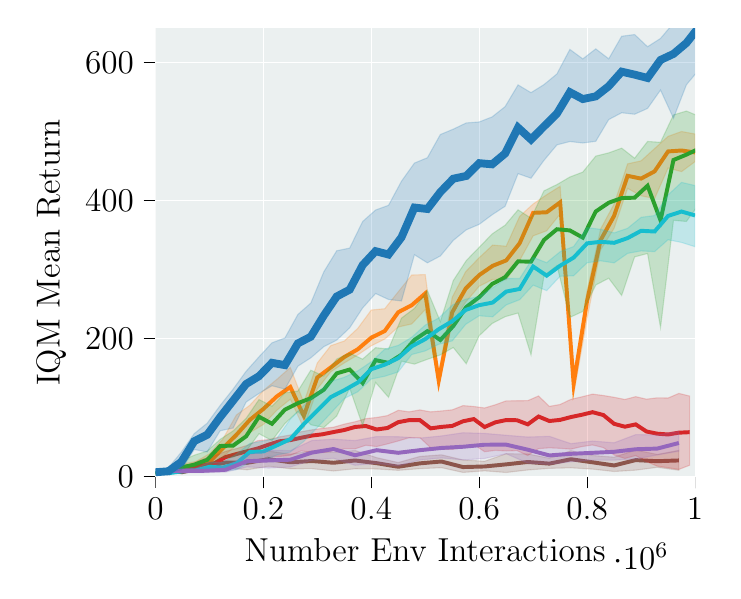
\begin{tikzpicture}

\definecolor{darkcyan1115178}{RGB}{1,115,178}
\definecolor{darkgray176}{RGB}{176,176,176}

\begin{axis}[
legend cell align={left},
legend style={fill opacity=0.8, draw opacity=1, text opacity=1, draw=lightgray204, at={(0.03,0.03)},  anchor=north west},
tick align=outside,
tick pos=left,
x grid style={white},
xlabel={Number Env Interactions},
xmajorgrids,
%xmin=-37798.95, xmax=1045799.95,
xmin=-0.0, xmax=1000000.0,
xtick style={color=black},
y grid style={white},
ylabel={IQM Mean Return},
ymajorgrids,
ymin=-0.05, ymax=650,
ytick style={color=black},
axis background/.style={fill=plot_background},
label style={font=\large},
tick label style={font=\large},
x axis line style={draw=none},
y axis line style={draw=none},
]
%Consistency-AC
\path [draw=C5, fill=C5, opacity=0.2]
(axis cs:10000,11.463926848519)
--(axis cs:10000,5.37603210746611)
--(axis cs:50000,4.39841287621437)
--(axis cs:90000,9.17009640948666)
--(axis cs:130000,12.5870741668558)
--(axis cs:170000,9.68308216662577)
--(axis cs:210000,14.8925226931926)
--(axis cs:250000,11.1820716312957)
--(axis cs:290000,11.396756534118)
--(axis cs:330000,7.99325851842966)
--(axis cs:370000,11.1976030725659)
--(axis cs:410000,10.9248649239103)
--(axis cs:450000,8.95682571708669)
--(axis cs:490000,11.3816416377384)
--(axis cs:530000,12.8031758180575)
--(axis cs:570000,5.93578222734027)
--(axis cs:610000,8.21484428635898)
--(axis cs:650000,5.83358756157396)
--(axis cs:690000,9.46063935999991)
--(axis cs:730000,11.8192892604622)
--(axis cs:770000,12.6324885084212)
--(axis cs:810000,10.7473805476358)
--(axis cs:850000,7.25710635201092)
--(axis cs:890000,9.22131175112653)
--(axis cs:930000,13.2959293771329)
--(axis cs:970000,9.07029053354509)
--(axis cs:970000,37.8713919076384)
--(axis cs:970000,37.8713919076384)
--(axis cs:930000,31.9938327977292)
--(axis cs:890000,38.3203005660843)
--(axis cs:850000,28.0270492957679)
--(axis cs:810000,30.4347320062739)
--(axis cs:770000,37.3854786322548)
--(axis cs:730000,26.5349621208757)
--(axis cs:690000,32.7462369505973)
--(axis cs:650000,32.9976763829575)
--(axis cs:610000,22.0810080347503)
--(axis cs:570000,23.99523732983)
--(axis cs:530000,31.4375655225092)
--(axis cs:490000,29.0553190783567)
--(axis cs:450000,20.2524552334538)
--(axis cs:410000,27.2952511671052)
--(axis cs:370000,37.7092802874593)
--(axis cs:330000,34.8692907577358)
--(axis cs:290000,37.059821440363)
--(axis cs:250000,32.3343063705168)
--(axis cs:210000,36.8449215660586)
--(axis cs:170000,35.6687195813457)
--(axis cs:130000,28.0108828768184)
--(axis cs:90000,16.3792435674084)
--(axis cs:50000,9.69504458234381)
--(axis cs:10000,11.463926848519)
--cycle;

\addplot [line width=\linewidthother, C5, mark=*, mark size=0, mark options={solid}]
table {%
10000 7.85790325056077
50000 6.35860284032434
90000 13.2047146607297
130000 20.2989785218371
170000 19.8783841188691
210000 25.1934057825873
250000 20.6458589247297
290000 22.4396386818743
330000 19.9098415026298
370000 23.2276422103183
410000 19.3148549082268
450000 14.1367493320261
490000 19.0624373739155
530000 21.7560782762676
570000 13.6733204746371
610000 14.5346796841287
650000 17.6235735715368
690000 21.0359604016945
730000 18.6881061488316
770000 25.008983570338
810000 20.5910562769549
850000 16.0209033037917
890000 23.7708061586054
930000 22.2085724808314
970000 23.2810248149431
};

% BRO
\path [draw=C1, fill=C1, opacity=0.2]
(axis cs:25000,10.4214828010349)
--(axis cs:25000,5.74333818509858)
--(axis cs:50000,8.09432444087523)
--(axis cs:75000,9.90836608721418)
--(axis cs:100000,13.4284553407894)
--(axis cs:125000,28.5942453949379)
--(axis cs:150000,45.3514736374534)
--(axis cs:175000,63.5466645826227)
--(axis cs:200000,75.4050965367814)
--(axis cs:225000,96.0977329143482)
--(axis cs:250000,112.144633001037)
--(axis cs:275000,69.758808886236)
--(axis cs:300000,126.88587225159)
--(axis cs:325000,151.854080295755)
--(axis cs:350000,164.689782841864)
--(axis cs:375000,176.267798146898)
--(axis cs:400000,189.528921194811)
--(axis cs:425000,199.237052941994)
--(axis cs:450000,216.76527008714)
--(axis cs:475000,221.172823432845)
--(axis cs:500000,242.047785506084)
--(axis cs:525000,131.845836334689)
--(axis cs:550000,223.08224577297)
--(axis cs:575000,252.840470629034)
--(axis cs:600000,275.886393376962)
--(axis cs:625000,285.859410268162)
--(axis cs:650000,285.091806186583)
--(axis cs:675000,313.370579224885)
--(axis cs:700000,348.91564649927)
--(axis cs:725000,356.289859109605)
--(axis cs:750000,380.482061980522)
--(axis cs:775000,118.739536778631)
--(axis cs:800000,229.14440596249)
--(axis cs:825000,328.406216187075)
--(axis cs:850000,360.007008496921)
--(axis cs:875000,417.747465127326)
--(axis cs:900000,407.011657970625)
--(axis cs:925000,402.973664549389)
--(axis cs:950000,447.23319412658)
--(axis cs:975000,442.036693024441)
--(axis cs:1000000,456.581953317235)
--(axis cs:1000000,496.59024771113)
--(axis cs:1000000,496.59024771113)
--(axis cs:975000,500.244726881671)
--(axis cs:950000,493.170094491512)
--(axis cs:925000,475.46384217299)
--(axis cs:900000,457.711206302229)
--(axis cs:875000,453.350626938457)
--(axis cs:850000,395.073608046901)
--(axis cs:825000,358.933679864953)
--(axis cs:800000,269.559873348413)
--(axis cs:775000,143.266187556657)
--(axis cs:750000,420.817298900866)
--(axis cs:725000,408.555355122614)
--(axis cs:700000,395.166196894937)
--(axis cs:675000,377.23826528108)
--(axis cs:650000,333.916215702771)
--(axis cs:625000,335.57168171148)
--(axis cs:600000,317.262483428054)
--(axis cs:575000,297.120865242452)
--(axis cs:550000,259.923563574532)
--(axis cs:525000,150.311833808402)
--(axis cs:500000,292.772584457249)
--(axis cs:475000,292.135052782577)
--(axis cs:450000,267.872285614804)
--(axis cs:425000,243.291577456831)
--(axis cs:400000,241.393645358009)
--(axis cs:375000,214.800057235155)
--(axis cs:350000,196.464908151334)
--(axis cs:325000,189.755589772141)
--(axis cs:300000,164.593901002474)
--(axis cs:275000,107.111385050975)
--(axis cs:250000,158.16812429377)
--(axis cs:225000,140.832875677263)
--(axis cs:200000,124.605494930318)
--(axis cs:175000,103.327680424693)
--(axis cs:150000,89.2303886773787)
--(axis cs:125000,54.2583886820005)
--(axis cs:100000,32.8955349031664)
--(axis cs:75000,21.7858682309204)
--(axis cs:50000,18.1647642728865)
--(axis cs:25000,10.4214828010349)
--cycle;

\addplot [line width=\linewidthother, C1, mark=*, mark size=0, mark options={solid}]
table {%
25000 7.69078524526657
50000 12.7531337620864
75000 16.4813932058173
100000 20.9576496494661
125000 40.9559750123288
150000 60.3425381404668
175000 82.1009523487325
200000 97.9155570347124
225000 116.102735256329
250000 129.831786801786
275000 87.8189239900971
300000 143.560432818343
325000 158.198346748268
350000 173.236261187279
375000 184.46223583009
400000 201.289153423342
425000 211.007935561594
450000 238.189807796344
475000 248.385497862529
500000 265.493017462384
525000 138.929177278294
550000 238.047698713837
575000 272.57812456009
600000 292.037445610574
625000 305.485935589137
650000 313.27007681098
675000 338.308375304241
700000 382.29668702033
725000 383.13758244702
750000 397.500063267137
775000 134.47735028663
800000 254.98358315637
825000 342.750590156139
850000 377.967783546172
875000 435.965517877994
900000 431.952717196056
925000 442.435174817137
950000 471.334996063751
975000 472.695410507355
1000000 469.884836753752
};
% QSM
\path [draw=C3, fill=C3, opacity=0.2]
(axis cs:10000,9.00637129942576)
--(axis cs:10000,3.31341858704885)
--(axis cs:30000,5.57260828216871)
--(axis cs:50000,8.02879546334346)
--(axis cs:70000,8.96538097100953)
--(axis cs:90000,10.0447169281542)
--(axis cs:110000,11.083192997224)
--(axis cs:130000,15.8602566473863)
--(axis cs:150000,20.0827251935657)
--(axis cs:170000,21.7714599737985)
--(axis cs:190000,21.2784577034276)
--(axis cs:210000,29.2425191401357)
--(axis cs:230000,29.1000896614077)
--(axis cs:250000,30.7142972597102)
--(axis cs:270000,37.1213915977744)
--(axis cs:290000,35.383553986563)
--(axis cs:310000,34.5792193715324)
--(axis cs:330000,37.180703958727)
--(axis cs:350000,39.9991572830434)
--(axis cs:370000,40.0996391593703)
--(axis cs:390000,45.3179218579362)
--(axis cs:410000,43.4128867200092)
--(axis cs:430000,47.2341654755311)
--(axis cs:450000,51.4904100888942)
--(axis cs:470000,56.1438953381185)
--(axis cs:490000,56.3643598825837)
--(axis cs:510000,41.8560678676204)
--(axis cs:530000,39.4311747974906)
--(axis cs:550000,39.2973707636431)
--(axis cs:570000,42.1655587598545)
--(axis cs:590000,46.474886428713)
--(axis cs:610000,35.9292819193922)
--(axis cs:630000,37.867541948254)
--(axis cs:650000,37.0515135860717)
--(axis cs:670000,37.5128013938228)
--(axis cs:690000,30.5023094831127)
--(axis cs:710000,40.438926076983)
--(axis cs:730000,41.6069058038226)
--(axis cs:750000,40.8430295724723)
--(axis cs:770000,39.7151342713554)
--(axis cs:790000,43.331485201916)
--(axis cs:810000,45.728076310577)
--(axis cs:830000,41.9312130426918)
--(axis cs:850000,31.1859364236329)
--(axis cs:870000,26.1690699101898)
--(axis cs:890000,30.3492033461859)
--(axis cs:910000,21.6742292892421)
--(axis cs:930000,15.00353959044)
--(axis cs:950000,12.6778280563617)
--(axis cs:970000,10.276360763814)
--(axis cs:990000,16.3133930613083)
--(axis cs:990000,116.662159246092)
--(axis cs:990000,116.662159246092)
--(axis cs:970000,120.475571672727)
--(axis cs:950000,113.793179632632)
--(axis cs:930000,114.084972864025)
--(axis cs:910000,112.135332782087)
--(axis cs:890000,115.757407879623)
--(axis cs:870000,111.72505328964)
--(axis cs:850000,114.856922483414)
--(axis cs:830000,117.448915056765)
--(axis cs:810000,119.459803820126)
--(axis cs:790000,115.453403901555)
--(axis cs:770000,111.913551390986)
--(axis cs:750000,104.420705974677)
--(axis cs:730000,101.661488486193)
--(axis cs:710000,116.777563783003)
--(axis cs:690000,109.956826669484)
--(axis cs:670000,109.846564750774)
--(axis cs:650000,109.69722781989)
--(axis cs:630000,104.017540868934)
--(axis cs:610000,99.3662446587841)
--(axis cs:590000,101.502700353239)
--(axis cs:570000,102.777559600424)
--(axis cs:550000,96.6413273589876)
--(axis cs:530000,95.0563691400709)
--(axis cs:510000,93.7333309362891)
--(axis cs:490000,96.5183300919841)
--(axis cs:470000,93.7539031450182)
--(axis cs:450000,95.9979843577684)
--(axis cs:430000,88.2955526826802)
--(axis cs:410000,85.5825312019854)
--(axis cs:390000,83.9140755855183)
--(axis cs:370000,79.393379419303)
--(axis cs:350000,75.9247120943175)
--(axis cs:330000,71.4454448500963)
--(axis cs:310000,69.8080548912829)
--(axis cs:290000,67.6769566217011)
--(axis cs:270000,64.9307342505208)
--(axis cs:250000,60.1687479824038)
--(axis cs:230000,57.4818564634574)
--(axis cs:210000,53.5049428912655)
--(axis cs:190000,52.0394126697339)
--(axis cs:170000,45.0678509664825)
--(axis cs:150000,40.4675526829694)
--(axis cs:130000,36.4301813118218)
--(axis cs:110000,30.0792382984102)
--(axis cs:90000,25.7764486732582)
--(axis cs:70000,19.3209997828429)
--(axis cs:50000,13.7913653403521)
--(axis cs:30000,8.02777871837219)
--(axis cs:10000,9.00637129942576)
--cycle;


\addplot [line width=\linewidthother, C3, mark=*, mark size=0, mark options={solid}]
table {%
10000 5.48336112499237
30000 6.85617107152939
50000 10.2728418062131
70000 12.3853853059312
90000 16.2610089325656
110000 19.3796129614736
130000 28.1669670593013
150000 32.534822997574
170000 36.6120637002399
190000 40.751044902772
210000 46.2025473896589
230000 51.0763229516388
250000 52.771598438105
270000 56.1948414493802
290000 59.3300952228345
310000 61.2587398424496
330000 64.4361855497106
350000 67.4036484636402
370000 71.8194046238446
390000 73.2278073683228
410000 68.1734948966614
430000 70.3253361188797
450000 78.7786298544066
470000 81.7159956085398
490000 81.7640809562731
510000 69.7941905260474
530000 71.9224686126011
550000 73.348937141401
570000 80.0750538907225
590000 83.2811232275952
610000 71.7244561219077
630000 78.5604585154285
650000 81.8548987770866
670000 81.5800458606281
690000 75.6349773808369
710000 86.9667827749601
730000 80.4607181570385
750000 82.0978496071994
770000 86.2036625367779
790000 89.4833001638254
810000 93.2583586598661
830000 89.1554655603121
850000 76.3665210100897
870000 72.2112299010237
890000 75.572761595307
910000 65.2483546448566
930000 62.0938081454536
950000 60.9241431782228
970000 63.5439467565627
990000 64.2725527717772
};

\path [draw=C2, fill=C2, opacity=0.2]
(axis cs:1,5.08870304)
--(axis cs:1,3.68965048)
--(axis cs:24000,7.62991894)
--(axis cs:48000,7.93215652)
--(axis cs:72000,6.47293496650009)
--(axis cs:96000,12.587974)
--(axis cs:120000,27.3698494)
--(axis cs:144000,28.12897)
--(axis cs:168000,36.614457)
--(axis cs:192000,62.045424)
--(axis cs:216000,52.0521822)
--(axis cs:240000,76.786258)
--(axis cs:264000,94.280188)
--(axis cs:288000,74.9881499350004)
--(axis cs:312000,71.0480906)
--(axis cs:336000,87.6450248)
--(axis cs:360000,128.128906)
--(axis cs:384000,73.9193625100026)
--(axis cs:408000,136.3864164)
--(axis cs:432000,114.8276584)
--(axis cs:456000,167.233562)
--(axis cs:480000,162.955824)
--(axis cs:504000,169.927532)
--(axis cs:528000,176.322408)
--(axis cs:552000,187.024622)
--(axis cs:576000,163.487644)
--(axis cs:600000,204.19103)
--(axis cs:624000,221.893322)
--(axis cs:648000,231.709012)
--(axis cs:672000,236.976125050001)
--(axis cs:696000,176.3649328)
--(axis cs:720000,290.38816)
--(axis cs:744000,305.915814)
--(axis cs:768000,230.663312)
--(axis cs:792000,239.332844)
--(axis cs:816000,277.67124)
--(axis cs:840000,287.474624)
--(axis cs:864000,262.481308)
--(axis cs:888000,318.412994)
--(axis cs:912000,323.347184)
--(axis cs:936000,215.92877)
--(axis cs:960000,371.48532)
--(axis cs:984000,369.806744)
--(axis cs:1008000,395.842144)
--(axis cs:1032000,250.919718510006)
--(axis cs:1056000,411.625820300001)
--(axis cs:1080000,407.048594)
--(axis cs:1104000,419.546388)
--(axis cs:1128000,454.343112)
--(axis cs:1152000,268.321736)
--(axis cs:1176000,306.649356)
--(axis cs:1200000,473.455544)
--(axis cs:1224000,468.99469)
--(axis cs:1248000,392.569902)
--(axis cs:1272000,367.470216)
--(axis cs:1296000,514.64103)
--(axis cs:1320000,525.853924)
--(axis cs:1344000,523.617598)
--(axis cs:1368000,505.30544)
--(axis cs:1392000,481.589782)
--(axis cs:1416000,546.605916)
--(axis cs:1440000,549.00744)
--(axis cs:1464000,516.795564)
--(axis cs:1488000,530.279436)
--(axis cs:1512000,537.87598)
--(axis cs:1536000,583.42678)
--(axis cs:1560000,578.29042)
--(axis cs:1584000,349.135284)
--(axis cs:1608000,524.726164)
--(axis cs:1632000,598.62813)
--(axis cs:1656000,395.3759324)
--(axis cs:1680000,578.054076)
--(axis cs:1704000,368.5988572)
--(axis cs:1728000,560.359838)
--(axis cs:1752000,605.988216)
--(axis cs:1776000,616.570372)
--(axis cs:1800000,586.88821)
--(axis cs:1824000,608.40061)
--(axis cs:1848000,601.388426)
--(axis cs:1872000,599.06138)
--(axis cs:1896000,490.962722)
--(axis cs:1920000,276.865072)
--(axis cs:1944000,538.00442)
--(axis cs:1968000,646.4052)
--(axis cs:1992000,633.225998)
--(axis cs:2016000,639.749272)
--(axis cs:2040000,529.704108)
--(axis cs:2064000,657.623612)
--(axis cs:2088000,606.7978)
--(axis cs:2112000,557.042702)
--(axis cs:2136000,642.73752)
--(axis cs:2160000,645.962118)
--(axis cs:2184000,422.8458116)
--(axis cs:2208000,580.496716)
--(axis cs:2232000,687.99286)
--(axis cs:2256000,596.495068)
--(axis cs:2280000,688.213466)
--(axis cs:2304000,616.179208)
--(axis cs:2328000,581.54152)
--(axis cs:2352000,419.4881004)
--(axis cs:2376000,502.770992)
--(axis cs:2400000,600.524793000003)
--(axis cs:2424000,664.403404)
--(axis cs:2448000,627.83858)
--(axis cs:2472000,687.23751)
--(axis cs:2496000,597.76742)
--(axis cs:2520000,656.83965)
--(axis cs:2544000,526.801084)
--(axis cs:2568000,470.997188)
--(axis cs:2592000,636.76534)
--(axis cs:2616000,569.29958)
--(axis cs:2640000,672.796042)
--(axis cs:2664000,630.420594)
--(axis cs:2688000,550.655396)
--(axis cs:2712000,644.0207)
--(axis cs:2736000,589.857666)
--(axis cs:2760000,666.78616)
--(axis cs:2784000,617.303856)
--(axis cs:2808000,658.61183)
--(axis cs:2832000,682.914396)
--(axis cs:2856000,686.516124)
--(axis cs:2880000,710.847194)
--(axis cs:2904000,521.721572)
--(axis cs:2928000,504.00449)
--(axis cs:2952000,715.43871)
--(axis cs:2976000,609.043312)
--(axis cs:3000000,697.05923)
--(axis cs:3000000,816.05479)
--(axis cs:3000000,816.05479)
--(axis cs:2976000,816.833628)
--(axis cs:2952000,820.42984)
--(axis cs:2928000,802.37344)
--(axis cs:2904000,805.968666)
--(axis cs:2880000,797.86731)
--(axis cs:2856000,826.739952)
--(axis cs:2832000,806.72521)
--(axis cs:2808000,800.223108)
--(axis cs:2784000,817.777648)
--(axis cs:2760000,810.177492)
--(axis cs:2736000,804.11192)
--(axis cs:2712000,775.78706)
--(axis cs:2688000,798.70296)
--(axis cs:2664000,800.247196)
--(axis cs:2640000,806.08496)
--(axis cs:2616000,773.087792)
--(axis cs:2592000,757.598130200002)
--(axis cs:2568000,782.15722)
--(axis cs:2544000,792.273964)
--(axis cs:2520000,757.921734)
--(axis cs:2496000,748.993818)
--(axis cs:2472000,770.14045)
--(axis cs:2448000,748.8993)
--(axis cs:2424000,745.527544)
--(axis cs:2400000,743.45228)
--(axis cs:2376000,769.958568)
--(axis cs:2352000,718.61474)
--(axis cs:2328000,794.272146)
--(axis cs:2304000,802.248602)
--(axis cs:2280000,786.811476)
--(axis cs:2256000,760.0894)
--(axis cs:2232000,790.97057)
--(axis cs:2208000,775.016552)
--(axis cs:2184000,768.423152)
--(axis cs:2160000,743.21318)
--(axis cs:2136000,765.272132)
--(axis cs:2112000,759.624902)
--(axis cs:2088000,748.89576)
--(axis cs:2064000,745.63012)
--(axis cs:2040000,722.20737)
--(axis cs:2016000,743.0933)
--(axis cs:1992000,724.294948)
--(axis cs:1968000,752.22605)
--(axis cs:1944000,728.1269)
--(axis cs:1920000,730.239636)
--(axis cs:1896000,696.265756)
--(axis cs:1872000,716.48952)
--(axis cs:1848000,722.897252)
--(axis cs:1824000,700.40674)
--(axis cs:1800000,681.427446)
--(axis cs:1776000,702.65155)
--(axis cs:1752000,679.932826)
--(axis cs:1728000,679.549276)
--(axis cs:1704000,715.56346)
--(axis cs:1680000,688.76336)
--(axis cs:1656000,683.049632)
--(axis cs:1632000,693.61822)
--(axis cs:1608000,687.3224)
--(axis cs:1584000,651.290338)
--(axis cs:1560000,674.12986)
--(axis cs:1536000,675.877516)
--(axis cs:1512000,669.480454)
--(axis cs:1488000,638.062)
--(axis cs:1464000,662.310476)
--(axis cs:1440000,652.789328)
--(axis cs:1416000,651.846968)
--(axis cs:1392000,635.23482)
--(axis cs:1368000,635.917)
--(axis cs:1344000,635.4749)
--(axis cs:1320000,616.55244)
--(axis cs:1296000,619.092528)
--(axis cs:1272000,592.115148)
--(axis cs:1248000,585.497024)
--(axis cs:1224000,596.60722)
--(axis cs:1200000,594.4673)
--(axis cs:1176000,591.790048)
--(axis cs:1152000,549.044842)
--(axis cs:1128000,568.078136)
--(axis cs:1104000,576.72876)
--(axis cs:1080000,553.44684)
--(axis cs:1056000,546.617916)
--(axis cs:1032000,543.060196)
--(axis cs:1008000,522.083816)
--(axis cs:984000,529.931406)
--(axis cs:960000,524.29467)
--(axis cs:936000,484.517842)
--(axis cs:912000,485.825776)
--(axis cs:888000,461.478972)
--(axis cs:864000,476.117322)
--(axis cs:840000,469.27586)
--(axis cs:816000,464.6017)
--(axis cs:792000,441.409176)
--(axis cs:768000,434.262428)
--(axis cs:744000,423.281106)
--(axis cs:720000,414.170984)
--(axis cs:696000,374.5067)
--(axis cs:672000,386.673746)
--(axis cs:648000,364.314222)
--(axis cs:624000,351.766138)
--(axis cs:600000,332.345748)
--(axis cs:576000,313.014292)
--(axis cs:552000,284.177572)
--(axis cs:528000,224.632766)
--(axis cs:504000,269.586118)
--(axis cs:480000,243.80664)
--(axis cs:456000,229.6212)
--(axis cs:432000,184.839836)
--(axis cs:408000,186.79067)
--(axis cs:384000,170.161898)
--(axis cs:360000,178.871194)
--(axis cs:336000,170.301876)
--(axis cs:312000,145.5524092)
--(axis cs:288000,154.151556)
--(axis cs:264000,123.806023)
--(axis cs:240000,121.281625)
--(axis cs:216000,101.8625024)
--(axis cs:192000,111.603644)
--(axis cs:168000,84.20818)
--(axis cs:144000,66.140008)
--(axis cs:120000,53.8429784)
--(axis cs:96000,36.8297434)
--(axis cs:72000,30.9384382)
--(axis cs:48000,22.3311096)
--(axis cs:24000,12.7853277)
--(axis cs:1,5.08870304)
--cycle;

\addplot [line width=\linewidthother, C2, mark=*, mark size=0, mark options={solid}]
table {%
1 4.482758
24000 8.95052342
48000 13.292312
72000 17.10010038
96000 24.2130636
120000 44.2345288
144000 44.805972
168000 58.174146
192000 86.655458
216000 76.4512708
240000 96.9551522
264000 106.345815
288000 113.5489152
312000 125.7857092
336000 149.555445
360000 155.09633
384000 135.472366
408000 168.755284
432000 164.716176
456000 176.57803
480000 198.114586
504000 210.71531
528000 197.930814
552000 218.164982
576000 245.695396
600000 260.076062
624000 279.168826
648000 288.94217
672000 311.86936
696000 311.543426
720000 342.935496
744000 358.51124
768000 356.785058
792000 346.377912
816000 384.285682
840000 396.962226
864000 403.701502
888000 404.300138
912000 421.602336
936000 371.433818
960000 458.90596
984000 466.7362
1008000 475.609888
1032000 439.628622
1056000 485.556884
1080000 486.492076
1104000 505.164156
1128000 504.46871
1152000 461.414462
1176000 503.718468
1200000 522.697416
1224000 527.268044
1248000 506.490704
1272000 510.735564
1296000 559.11353
1320000 569.6844
1344000 569.031614
1368000 555.68144
1392000 583.679534
1416000 589.009554
1440000 594.783848
1464000 590.90014
1488000 570.207448
1512000 614.117482
1536000 619.260512
1560000 610.24442
1584000 569.768914
1608000 629.699378
1632000 634.41287
1656000 609.00341
1680000 635.959072
1704000 633.569498
1728000 623.042454
1752000 639.838396
1776000 648.812748
1800000 617.114056
1824000 647.1812
1848000 656.620386
1872000 660.19625
1896000 620.346456
1920000 554.823928
1944000 630.0526
1968000 686.13246
1992000 674.612466
2016000 680.493322
2040000 656.338942
2064000 694.551632
2088000 681.743874
2112000 701.884236
2136000 702.578264
2160000 692.050634
2184000 698.019532
2208000 715.948058
2232000 733.527184
2256000 682.839552
2280000 732.036794
2304000 720.45979
2328000 736.558496
2352000 663.161484
2376000 720.5217
2400000 697.58044
2424000 708.987852
2448000 691.49205
2472000 724.504812
2496000 700.70355
2520000 701.45418
2544000 734.79906
2568000 747.058346
2592000 725.77554
2616000 725.551706
2640000 748.126478
2664000 738.848702
2688000 730.628632
2712000 701.435
2736000 745.88346
2760000 753.473008
2784000 737.01486
2808000 750.083314
2832000 739.435622
2856000 762.29916
2880000 743.762224
2904000 739.993606
2928000 735.47718
2952000 777.263996
2976000 747.561014
3000000 765.32302
};

%BRO FAST 
\path [draw=C9, fill=C9, opacity=0.2]
(axis cs:25000,5.9627663029069)
--(axis cs:25000,3.94060263678752)
--(axis cs:50000,4.95329533063607)
--(axis cs:75000,7.2229154274937)
--(axis cs:100000,8.99076950219844)
--(axis cs:125000,7.88746522576995)
--(axis cs:150000,9.9448038857203)
--(axis cs:175000,20.6593185029793)
--(axis cs:200000,23.0857594811648)
--(axis cs:225000,31.1824613187434)
--(axis cs:250000,35.3533155525059)
--(axis cs:275000,50.8855500678719)
--(axis cs:300000,70.896840543864)
--(axis cs:325000,91.822405905343)
--(axis cs:350000,113.084879165756)
--(axis cs:375000,122.774920886158)
--(axis cs:400000,141.378469992151)
--(axis cs:425000,145.33166528664)
--(axis cs:450000,151.666671178168)
--(axis cs:475000,176.85704034099)
--(axis cs:500000,182.085180871627)
--(axis cs:525000,191.751877225063)
--(axis cs:550000,196.599502475127)
--(axis cs:575000,220.690109788465)
--(axis cs:600000,233.046428298572)
--(axis cs:625000,231.563550852072)
--(axis cs:650000,248.772572748877)
--(axis cs:675000,256.393197597437)
--(axis cs:700000,277.473464178774)
--(axis cs:725000,269.557616819856)
--(axis cs:750000,290.371096291129)
--(axis cs:775000,291.060337269253)
--(axis cs:800000,309.919693983718)
--(axis cs:825000,312.742653871502)
--(axis cs:850000,309.756613917194)
--(axis cs:875000,323.530706851565)
--(axis cs:900000,327.138909058089)
--(axis cs:925000,326.036401919083)
--(axis cs:950000,343.340258361995)
--(axis cs:975000,339.367940478116)
--(axis cs:1000000,333.206963775736)
--(axis cs:1000000,421.840029904296)
--(axis cs:1000000,421.840029904296)
--(axis cs:975000,426.477170525367)
--(axis cs:950000,408.366883033887)
--(axis cs:925000,378.320544206267)
--(axis cs:900000,375.814281035147)
--(axis cs:875000,359.889404656802)
--(axis cs:850000,353.210436290579)
--(axis cs:825000,358.3961066085)
--(axis cs:800000,360.80720507426)
--(axis cs:775000,333.439747195314)
--(axis cs:750000,325.96784250545)
--(axis cs:725000,310.065576884353)
--(axis cs:700000,317.662111605769)
--(axis cs:675000,287.03975300699)
--(axis cs:650000,287.166302214974)
--(axis cs:625000,273.632184905015)
--(axis cs:600000,260.860218679205)
--(axis cs:575000,257.138188475866)
--(axis cs:550000,248.544989304806)
--(axis cs:525000,229.709147298703)
--(axis cs:500000,219.532839209569)
--(axis cs:475000,201.932086693417)
--(axis cs:450000,190.087953115992)
--(axis cs:425000,184.630699497815)
--(axis cs:400000,166.354795684718)
--(axis cs:375000,153.138164951746)
--(axis cs:350000,143.826268523414)
--(axis cs:325000,137.892671673645)
--(axis cs:300000,121.06169983147)
--(axis cs:275000,103.340431962028)
--(axis cs:250000,83.169536368522)
--(axis cs:225000,55.4017394189915)
--(axis cs:200000,51.3296215803654)
--(axis cs:175000,48.0146769335392)
--(axis cs:150000,32.2985969187401)
--(axis cs:125000,20.4689000428325)
--(axis cs:100000,20.8867322996787)
--(axis cs:75000,11.996196520421)
--(axis cs:50000,10.8775441795892)
--(axis cs:25000,5.9627663029069)
--cycle;

\addplot [line width=\linewidthother, C9, mark=*, mark size=0, mark options={solid}]
table {%
25000 4.76931211996678
50000 7.75830953287283
75000 8.77929464496367
100000 14.0284487422699
125000 12.9102899220444
150000 18.8464043718836
175000 35.6132009401844
200000 36.2773846135605
225000 45.1248353278597
250000 54.2267690563538
275000 75.9807331931164
300000 95.4707102928311
325000 115.161371324838
350000 125.108995868431
375000 136.23022767119
400000 155.6035762322
425000 162.172617805304
450000 171.636124694723
475000 188.793437151646
500000 199.208471490115
525000 213.545280886908
550000 225.127755950347
575000 241.517190907147
600000 248.454736402755
625000 252.222876139156
650000 268.133074430179
675000 271.934776224982
700000 304.489538089164
725000 291.238290843002
750000 305.63835994789
775000 317.393607025809
800000 338.060161910782
825000 340.309283163538
850000 338.836958460671
875000 345.69471729392
900000 356.261290709827
925000 355.250340096369
950000 377.839546363
975000 384.180677473021
1000000 378.582505837938
};

%Diff-QL
\path [draw=C4, fill=C4, opacity=0.2]
(axis cs:10000,10.2812425960027)
--(axis cs:10000,6.02198363619497)
--(axis cs:50000,5.6899344243029)
--(axis cs:90000,5.71575920360953)
--(axis cs:130000,6.37500854819906)
--(axis cs:170000,13.928629817174)
--(axis cs:210000,12.2830882066452)
--(axis cs:250000,13.7931790285666)
--(axis cs:290000,23.6162004623858)
--(axis cs:330000,26.429559016189)
--(axis cs:370000,16.2833425090443)
--(axis cs:410000,19.0172584116363)
--(axis cs:450000,15.4066594707813)
--(axis cs:490000,23.9038833711864)
--(axis cs:530000,26.9407819846307)
--(axis cs:570000,24.0161717051929)
--(axis cs:610000,26.1196342836227)
--(axis cs:650000,32.9924744002448)
--(axis cs:690000,19.4350844063726)
--(axis cs:730000,17.6448948034238)
--(axis cs:770000,21.3235667429693)
--(axis cs:810000,23.7898332859306)
--(axis cs:850000,23.7954429329512)
--(axis cs:890000,25.4711678656995)
--(axis cs:930000,31.1899759133195)
--(axis cs:970000,36.6733448204817)
--(axis cs:970000,65.3130953140278)
--(axis cs:970000,65.3130953140278)
--(axis cs:930000,60.3616330092323)
--(axis cs:890000,60.697914227961)
--(axis cs:850000,48.8677851258972)
--(axis cs:810000,51.4295290804306)
--(axis cs:770000,47.6241784873465)
--(axis cs:730000,58.2453930520975)
--(axis cs:690000,57.2006607227685)
--(axis cs:650000,59.7837199585962)
--(axis cs:610000,62.4661212285104)
--(axis cs:570000,63.4328975323346)
--(axis cs:530000,58.8109865624696)
--(axis cs:490000,55.6746825931867)
--(axis cs:450000,57.6806297741792)
--(axis cs:410000,57.8697332277704)
--(axis cs:370000,52.1146904114954)
--(axis cs:330000,54.0363416001345)
--(axis cs:290000,52.2557397828543)
--(axis cs:250000,37.4225579324461)
--(axis cs:210000,38.2435984905139)
--(axis cs:170000,30.8571610481571)
--(axis cs:130000,15.2134009864936)
--(axis cs:90000,12.7719523040756)
--(axis cs:50000,11.3986260605429)
--(axis cs:10000,10.2812425960027)
--cycle;

\addplot [line width = \linewidthother, C4, mark=*, mark size=0, mark options={solid}]
table {%
10000 7.89490776182443
50000 7.9854333311754
90000 8.28937577211643
130000 9.77283196987029
170000 22.2536935035431
210000 23.2246065851491
250000 24.3473219356756
290000 34.6478363417292
330000 39.8473491621079
370000 30.8162680243438
410000 38.1505004392581
450000 34.3586620840302
490000 38.1543728235634
530000 41.383479841911
570000 43.1274020679081
610000 46.0577781009326
650000 46.1689029271184
690000 38.8777959370311
730000 30.5554718391215
770000 32.88675893705
810000 34.3310860617031
850000 35.8325598568167
890000 39.505923992965
930000 40.4884218643146
970000 48.59123916707
};

%DIME
\path [draw=C0, fill=C0, opacity=0.2]
(axis cs:1,6.80215591666667)
--(axis cs:1,5.5925808)
--(axis cs:24000,4.88713573333333)
--(axis cs:48000,9.748871)
--(axis cs:72000,39.178405)
--(axis cs:96000,35.577766)
--(axis cs:120000,66.3638765)
--(axis cs:144000,70.247577)
--(axis cs:168000,107.848963333333)
--(axis cs:192000,120.425612666667)
--(axis cs:216000,131.606081666667)
--(axis cs:240000,126.6783995)
--(axis cs:264000,159.943133333333)
--(axis cs:288000,172.044628333333)
--(axis cs:312000,188.191985)
--(axis cs:336000,197.75034)
--(axis cs:360000,215.573404333333)
--(axis cs:384000,244.38039)
--(axis cs:408000,265.35188)
--(axis cs:432000,256.659486666667)
--(axis cs:456000,254.555695)
--(axis cs:480000,321.560075)
--(axis cs:504000,309.784411666667)
--(axis cs:528000,319.716291666667)
--(axis cs:552000,342.35053)
--(axis cs:576000,357.640175)
--(axis cs:600000,365.597093333333)
--(axis cs:624000,379.492581666667)
--(axis cs:648000,391.800683333333)
--(axis cs:672000,439.1368195)
--(axis cs:696000,432.521263333333)
--(axis cs:720000,458.362536666667)
--(axis cs:744000,480.79676)
--(axis cs:768000,485.700503333333)
--(axis cs:792000,483.583248791667)
--(axis cs:816000,485.992758916667)
--(axis cs:840000,517.541645)
--(axis cs:864000,527.38718)
--(axis cs:888000,525.263277708333)
--(axis cs:912000,533.699495)
--(axis cs:936000,560.338303333333)
--(axis cs:960000,519.453665)
--(axis cs:984000,568.020833333333)
--(axis cs:1008000,590.470613333333)
--(axis cs:1032000,581.025416666667)
--(axis cs:1056000,583.688265)
--(axis cs:1080000,607.528891666667)
--(axis cs:1104000,620.278735)
--(axis cs:1128000,613.026586666667)
--(axis cs:1152000,638.844431666667)
--(axis cs:1176000,637.409991666667)
--(axis cs:1200000,641.941126666667)
--(axis cs:1224000,658.54966)
--(axis cs:1248000,646.231282291667)
--(axis cs:1272000,671.152858333333)
--(axis cs:1296000,660.192991666667)
--(axis cs:1320000,670.868964125)
--(axis cs:1344000,672.098633333333)
--(axis cs:1368000,667.270646666667)
--(axis cs:1392000,679.406895)
--(axis cs:1416000,667.768826166667)
--(axis cs:1440000,699.8657)
--(axis cs:1464000,703.368514541667)
--(axis cs:1488000,691.688456666667)
--(axis cs:1512000,691.02705)
--(axis cs:1536000,724.245045)
--(axis cs:1560000,642.1076)
--(axis cs:1584000,677.059261666667)
--(axis cs:1608000,722.467075)
--(axis cs:1632000,724.970475)
--(axis cs:1656000,707.042333333333)
--(axis cs:1680000,723.18196)
--(axis cs:1704000,739.733563333333)
--(axis cs:1728000,732.09224)
--(axis cs:1752000,743.118561666667)
--(axis cs:1776000,697.080626666666)
--(axis cs:1800000,709.36812)
--(axis cs:1824000,650.052771666667)
--(axis cs:1848000,716.700755)
--(axis cs:1872000,731.219691458333)
--(axis cs:1896000,703.767975)
--(axis cs:1920000,748.827876666667)
--(axis cs:1944000,769.246855)
--(axis cs:1968000,752.894191666667)
--(axis cs:1992000,737.845081666667)
--(axis cs:2016000,756.439925)
--(axis cs:2040000,764.171413333333)
--(axis cs:2064000,740.270250333333)
--(axis cs:2088000,725.118516666667)
--(axis cs:2112000,743.246291625)
--(axis cs:2136000,734.83942)
--(axis cs:2160000,786.861907708333)
--(axis cs:2184000,738.508053333333)
--(axis cs:2208000,750.911366666667)
--(axis cs:2232000,786.895078333333)
--(axis cs:2256000,798.218891666667)
--(axis cs:2280000,758.322531666667)
--(axis cs:2304000,768.420973333333)
--(axis cs:2328000,798.43544325)
--(axis cs:2352000,735.766616666667)
--(axis cs:2376000,763.731855)
--(axis cs:2400000,788.471761666667)
--(axis cs:2424000,798.863623333333)
--(axis cs:2448000,797.623013333333)
--(axis cs:2472000,798.009976666667)
--(axis cs:2496000,799.156973333333)
--(axis cs:2520000,789.180108333333)
--(axis cs:2544000,793.308771666667)
--(axis cs:2568000,766.555433333333)
--(axis cs:2592000,775.906533333333)
--(axis cs:2616000,657.870696541667)
--(axis cs:2640000,802.967105)
--(axis cs:2664000,762.239025)
--(axis cs:2688000,758.85175)
--(axis cs:2712000,832.457286666667)
--(axis cs:2736000,798.855305)
--(axis cs:2760000,790.104215)
--(axis cs:2784000,817.637935)
--(axis cs:2808000,791.100776666667)
--(axis cs:2832000,821.486588458333)
--(axis cs:2856000,798.389748333333)
--(axis cs:2880000,756.81125)
--(axis cs:2904000,809.53344)
--(axis cs:2928000,784.753078333333)
--(axis cs:2952000,778.719458333333)
--(axis cs:2976000,756.92755)
--(axis cs:3000000,792.897486666667)
--(axis cs:3000000,837.456603333333)
--(axis cs:3000000,837.456603333333)
--(axis cs:2976000,848.466266666667)
--(axis cs:2952000,849.20779)
--(axis cs:2928000,842.088306666667)
--(axis cs:2904000,854.474571666667)
--(axis cs:2880000,849.331893333333)
--(axis cs:2856000,862.497737875)
--(axis cs:2832000,869.625008333333)
--(axis cs:2808000,863.616378333333)
--(axis cs:2784000,860.982908333333)
--(axis cs:2760000,837.8695)
--(axis cs:2736000,852.905353333333)
--(axis cs:2712000,861.954153333333)
--(axis cs:2688000,830.469433333333)
--(axis cs:2664000,868.63305)
--(axis cs:2640000,864.472063333333)
--(axis cs:2616000,836.439531666667)
--(axis cs:2592000,863.806)
--(axis cs:2568000,856.3503)
--(axis cs:2544000,854.31376)
--(axis cs:2520000,848.667223333333)
--(axis cs:2496000,852.5053125)
--(axis cs:2472000,847.29574)
--(axis cs:2448000,844.57391)
--(axis cs:2424000,851.800331666667)
--(axis cs:2400000,842.753173333333)
--(axis cs:2376000,851.53189)
--(axis cs:2352000,824.298165)
--(axis cs:2328000,854.002923333333)
--(axis cs:2304000,823.149833333333)
--(axis cs:2280000,842.485828333333)
--(axis cs:2256000,850.53472)
--(axis cs:2232000,834.622511666667)
--(axis cs:2208000,832.830438333333)
--(axis cs:2184000,829.092180333333)
--(axis cs:2160000,843.589423333333)
--(axis cs:2136000,835.928383333333)
--(axis cs:2112000,828.188466666667)
--(axis cs:2088000,834.338206875)
--(axis cs:2064000,847.99647)
--(axis cs:2040000,817.802191666667)
--(axis cs:2016000,831.623071666667)
--(axis cs:1992000,808.728928708333)
--(axis cs:1968000,824.828883333333)
--(axis cs:1944000,821.340061666667)
--(axis cs:1920000,826.504741666667)
--(axis cs:1896000,818.318428333333)
--(axis cs:1872000,831.390226666667)
--(axis cs:1848000,826.4945)
--(axis cs:1824000,819.049933333333)
--(axis cs:1800000,842.232765791667)
--(axis cs:1776000,826.921123333333)
--(axis cs:1752000,834.800166666667)
--(axis cs:1728000,837.246975)
--(axis cs:1704000,853.61177)
--(axis cs:1680000,810.376866666667)
--(axis cs:1656000,808.423789083334)
--(axis cs:1632000,821.8582)
--(axis cs:1608000,815.354633333333)
--(axis cs:1584000,808.92544)
--(axis cs:1560000,812.104926666667)
--(axis cs:1536000,809.656291666667)
--(axis cs:1512000,782.288026666667)
--(axis cs:1488000,778.782291583334)
--(axis cs:1464000,778.858313333333)
--(axis cs:1440000,821.10777)
--(axis cs:1416000,783.881986666667)
--(axis cs:1392000,750.93809425)
--(axis cs:1368000,760.521313333333)
--(axis cs:1344000,766.813391666667)
--(axis cs:1320000,745.988075)
--(axis cs:1296000,745.58748175)
--(axis cs:1272000,778.078543333333)
--(axis cs:1248000,739.945458333333)
--(axis cs:1224000,752.028946666667)
--(axis cs:1200000,754.479292041667)
--(axis cs:1176000,738.838393333333)
--(axis cs:1152000,730.995366666667)
--(axis cs:1128000,726.874316666667)
--(axis cs:1104000,706.711063333333)
--(axis cs:1080000,710.372623333333)
--(axis cs:1056000,691.064566666667)
--(axis cs:1032000,651.101731666667)
--(axis cs:1008000,694.859348333333)
--(axis cs:984000,679.811011666667)
--(axis cs:960000,657.437975)
--(axis cs:936000,635.207354333333)
--(axis cs:912000,623.17085)
--(axis cs:888000,640.82537)
--(axis cs:864000,638.372956666667)
--(axis cs:840000,605.636066666667)
--(axis cs:816000,620.0484)
--(axis cs:792000,605.530201666667)
--(axis cs:768000,619.288428333333)
--(axis cs:744000,583.706463333333)
--(axis cs:720000,568.233463333333)
--(axis cs:696000,556.574435)
--(axis cs:672000,567.827056666667)
--(axis cs:648000,536.300349125)
--(axis cs:624000,521.473436666667)
--(axis cs:600000,514.082965)
--(axis cs:576000,512.673896666667)
--(axis cs:552000,503.68212)
--(axis cs:528000,495.859381666667)
--(axis cs:504000,462.220926666667)
--(axis cs:480000,454.484963333333)
--(axis cs:456000,428.183936666667)
--(axis cs:432000,393.258111666667)
--(axis cs:408000,386.389815)
--(axis cs:384000,369.733846666667)
--(axis cs:360000,331.193968333333)
--(axis cs:336000,327.351346666667)
--(axis cs:312000,296.701976666667)
--(axis cs:288000,251.529673375)
--(axis cs:264000,234.932268333333)
--(axis cs:240000,200.893656666667)
--(axis cs:216000,193.835535)
--(axis cs:192000,173.552272666667)
--(axis cs:168000,152.488876666667)
--(axis cs:144000,126.71998265)
--(axis cs:120000,102.995841)
--(axis cs:96000,77.3036046666667)
--(axis cs:72000,62.1926506666667)
--(axis cs:48000,35.3083526666667)
--(axis cs:24000,12.7237687833333)
--(axis cs:1,6.80215591666667)
--cycle;

\addplot [line width=\linewidthdime, C0, mark=*, mark size=0, mark options={solid}]
table {%
1 6.17641296666667
24000 7.56386268333333
48000 21.194537
72000 51.2078703333333
96000 60.4982363333333
120000 86.1485583333333
144000 110.007961666667
168000 134.059945
192000 145.492449333333
216000 164.83243
240000 161.520515
264000 192.983695
288000 202.72266
312000 233.335831666667
336000 261.032931666667
360000 270.949796666667
384000 306.506178333333
408000 326.736271666667
432000 321.852778333333
456000 346.82201
480000 389.972858333333
504000 387.914375
528000 412.405621666667
552000 431.808476666667
576000 435.778751666667
600000 454.327343333333
624000 452.650095
648000 468.345228333333
672000 505.85564
696000 488.718146666667
720000 507.547415
744000 526.153453333333
768000 557.257588333333
792000 547.320155
816000 551.174743333333
840000 565.919836666667
864000 586.99087
888000 582.702056666667
912000 577.851651666667
936000 603.980191666667
960000 612.742416666667
984000 628.581438333333
1008000 652.547345
1032000 621.855605
1056000 653.459033333333
1080000 677.789983333333
1104000 677.092326666667
1128000 688.166816666667
1152000 696.043668333333
1176000 689.546143333333
1200000 707.716985
1224000 716.223413333333
1248000 695.373521666667
1272000 729.041578333333
1296000 711.299655
1320000 714.779295
1344000 720.93956
1368000 718.17746
1392000 720.170855
1416000 742.45139
1440000 767.977446666667
1464000 745.921991666667
1488000 741.981485
1512000 740.075188333334
1536000 776.043163333333
1560000 730.35288
1584000 745.76982
1608000 774.030058333333
1632000 786.423141666667
1656000 775.007413333333
1680000 767.966193333333
1704000 803.248776666667
1728000 795.057825
1752000 799.094
1776000 768.546685
1800000 785.936768333333
1824000 770.381045
1848000 778.163971666667
1872000 784.5074
1896000 775.084686666667
1920000 803.85685
1944000 802.98721
1968000 799.194371666667
1992000 777.64892
2016000 809.862228333333
2040000 802.882363333333
2064000 807.031923333333
2088000 792.892843333333
2112000 784.135861666667
2136000 799.080736666667
2160000 829.289918333333
2184000 812.669866666667
2208000 798.845955
2232000 810.922945
2256000 829.769393333333
2280000 808.989303333333
2304000 787.9255
2328000 834.55804
2352000 790.163291666667
2376000 809.844736666667
2400000 823.614375
2424000 829.909856666667
2448000 827.945956666667
2472000 830.88744
2496000 832.031106666667
2520000 821.356241666667
2544000 822.67606
2568000 821.050315
2592000 838.71875
2616000 819.876546666667
2640000 836.608795
2664000 842.476748333333
2688000 800.310716666667
2712000 848.692928333333
2736000 828.082728333333
2760000 814.163598333333
2784000 843.60977
2808000 840.753683333333
2832000 848.649233333333
2856000 840.45366
2880000 812.837433333333
2904000 839.813745
2928000 813.380873333333
2952000 813.313951666667
2976000 809.99765
3000000 818.333465
};
\end{axis}

\end{tikzpicture}
}
       \subcaption[]{DIME and GB on Dog Run}
       \label{fig::appendix_dog_rund_dbs}
    \end{minipage}\hfill
    \begin{minipage}[b]{0.33\textwidth}
        \centering
       \resizebox{1\textwidth}{!}{% This file was created with tikzplotlib v0.10.1.
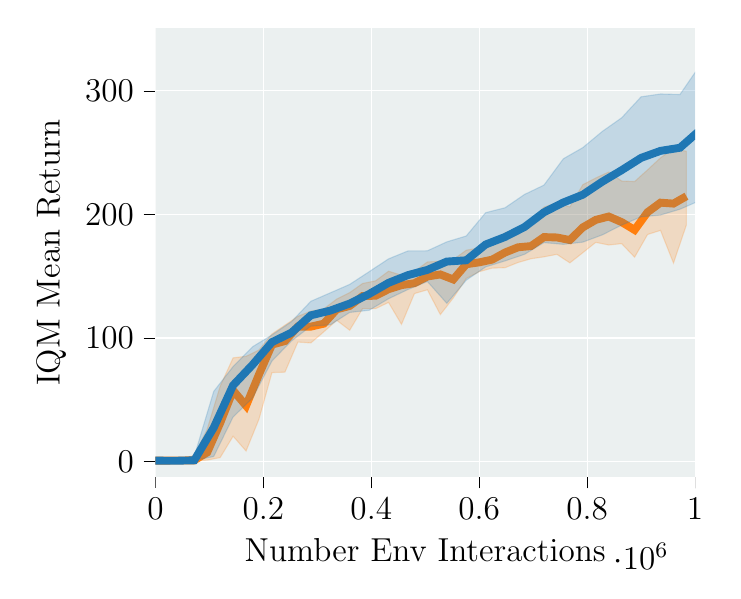
\begin{tikzpicture}

\definecolor{darkcyan1115178}{RGB}{1,115,178}
\definecolor{darkgray176}{RGB}{176,176,176}

\begin{axis}[
legend cell align={left},
legend cell align={left},
legend style={fill opacity=0.8, draw opacity=1, text opacity=1, draw=lightgray204, at={(0.5,0.03)},  anchor=south west},
tick align=outside,
tick pos=left,
x grid style={white},
xlabel={Number Env Interactions},
xmajorgrids,
xmin=-0.0, xmax=1000000.0,
xtick style={color=black},
y grid style={white},
ylabel={IQM Mean Return},
ymajorgrids,
ymin=-12.11232765065, ymax=350.65256879765,
ytick style={color=black},
axis background/.style={fill=plot_background},
label style={font=\large},
tick label style={font=\large},
x axis line style={draw=none},
y axis line style={draw=none},
]

\path [draw=C1, fill=C1, opacity=0.2]
(axis cs:1,0.913481333333333)
--(axis cs:1,0.6287236)
--(axis cs:24000,0.677781566666667)
--(axis cs:48000,0.738428966666667)
--(axis cs:72000,0.790174833333333)
--(axis cs:96000,1.1543524)
--(axis cs:120000,3.23502683000002)
--(axis cs:144000,20.5413528)
--(axis cs:168000,8.54387893333333)
--(axis cs:192000,34.4303118333333)
--(axis cs:216000,72.0098966666667)
--(axis cs:240000,72.3488675833333)
--(axis cs:264000,96.707165)
--(axis cs:288000,96.000784)
--(axis cs:312000,104.958421625)
--(axis cs:336000,114.297126)
--(axis cs:360000,106.284968)
--(axis cs:384000,123.7906925)
--(axis cs:408000,123.723489166667)
--(axis cs:432000,128.761211666667)
--(axis cs:456000,111.02938625)
--(axis cs:480000,135.956141666667)
--(axis cs:504000,138.98209)
--(axis cs:528000,118.929581333333)
--(axis cs:552000,132.387325)
--(axis cs:576000,148.148588333333)
--(axis cs:600000,153.61958)
--(axis cs:624000,156.55045)
--(axis cs:648000,156.870825)
--(axis cs:672000,161.074148333333)
--(axis cs:696000,164.107246666667)
--(axis cs:720000,165.654856541667)
--(axis cs:744000,167.669441666667)
--(axis cs:768000,160.786089)
--(axis cs:792000,168.99019)
--(axis cs:816000,177.369616666667)
--(axis cs:840000,175.239106666667)
--(axis cs:864000,176.361243333333)
--(axis cs:888000,165.394583333333)
--(axis cs:912000,183.752826666667)
--(axis cs:936000,187.066958333333)
--(axis cs:960000,160.625822716667)
--(axis cs:984000,191.555848333333)
--(axis cs:984000,251.074266666667)
--(axis cs:984000,251.074266666667)
--(axis cs:960000,253.124288333333)
--(axis cs:936000,245.776626666667)
--(axis cs:912000,236.034463333333)
--(axis cs:888000,226.598225)
--(axis cs:864000,227.013098708333)
--(axis cs:840000,234.283123333333)
--(axis cs:816000,229.472495)
--(axis cs:792000,224.034361666667)
--(axis cs:768000,206.047165)
--(axis cs:744000,209.549365)
--(axis cs:720000,205.859246666667)
--(axis cs:696000,194.984201666667)
--(axis cs:672000,188.552526666667)
--(axis cs:648000,185.157259583333)
--(axis cs:624000,177.684235)
--(axis cs:600000,172.894043333333)
--(axis cs:576000,171.0584)
--(axis cs:552000,163.391113333333)
--(axis cs:528000,162.135815)
--(axis cs:504000,161.517217666667)
--(axis cs:480000,153.846013166667)
--(axis cs:456000,150.815503333333)
--(axis cs:432000,154.043445)
--(axis cs:408000,146.23077)
--(axis cs:384000,144.130305)
--(axis cs:360000,136.713208333333)
--(axis cs:336000,131.509801666667)
--(axis cs:312000,123.557279541667)
--(axis cs:288000,121.774874166667)
--(axis cs:264000,117.476811666667)
--(axis cs:240000,110.350656666667)
--(axis cs:216000,103.274480333333)
--(axis cs:192000,90.3314516666667)
--(axis cs:168000,85.1717466666667)
--(axis cs:144000,83.9523868333333)
--(axis cs:120000,60.989724)
--(axis cs:96000,26.2789549666667)
--(axis cs:72000,5.35472753333333)
--(axis cs:48000,1.06001243333333)
--(axis cs:24000,0.923337466666667)
--(axis cs:1,0.913481333333333)
--cycle;

\addplot [line width=\linewidthdime, C1, mark=*, mark size=0, mark options={solid}]
table {%
1 0.7694417
24000 0.813880766666667
48000 0.903083466666667
72000 0.985341633333333
96000 7.39312896666667
120000 31.2267919666667
144000 57.5656945
168000 45.1603116666667
192000 70.5692
216000 94.6452396666667
240000 97.5139125
264000 109.186628333333
288000 109.1955065
312000 111.598211666667
336000 123.198625
360000 125.946167
384000 133.888621666667
408000 134.214293333333
432000 139.483735
456000 142.763216666667
480000 144.338755
504000 149.75221
528000 151.421726666667
552000 147.365006666667
576000 159.676698333333
600000 161.191491666667
624000 163.406718333333
648000 169.18849
672000 173.390193333333
696000 174.364796666667
720000 181.648728333333
744000 181.343818333333
768000 179.253028333333
792000 189.492575
816000 195.565436666667
840000 198.284515
864000 193.75859
888000 187.434418333333
912000 201.805691666667
936000 209.501925
960000 208.739933333333
984000 214.710998333333
};

%DIME
\path [draw=C0, fill=C0, opacity=0.2]
(axis cs:1,0.915501966666667)
--(axis cs:1,0.633556866666667)
--(axis cs:36000,0.5493304)
--(axis cs:72000,0.843873266666667)
--(axis cs:108000,4.13696455)
--(axis cs:144000,36.1211871666667)
--(axis cs:180000,51.4064937333333)
--(axis cs:216000,81.368514)
--(axis cs:252000,97.5408251666667)
--(axis cs:288000,109.583571666667)
--(axis cs:324000,110.618288333333)
--(axis cs:360000,120.684184666667)
--(axis cs:396000,122.417020833333)
--(axis cs:432000,131.747461666667)
--(axis cs:468000,139.23245)
--(axis cs:504000,145.708203333333)
--(axis cs:540000,128.071794166667)
--(axis cs:576000,146.743565)
--(axis cs:612000,157.523090333333)
--(axis cs:648000,162.386513333333)
--(axis cs:684000,167.712168333333)
--(axis cs:720000,177.17324)
--(axis cs:756000,175.778066666667)
--(axis cs:792000,177.557476666667)
--(axis cs:828000,183.413371666667)
--(axis cs:864000,191.343878333333)
--(axis cs:900000,198.058078333333)
--(axis cs:936000,199.495351666667)
--(axis cs:972000,204.18452)
--(axis cs:1008000,211.017165)
--(axis cs:1044000,210.395921666667)
--(axis cs:1080000,225.37889)
--(axis cs:1116000,225.57669)
--(axis cs:1152000,229.055506666667)
--(axis cs:1188000,244.717408333333)
--(axis cs:1224000,235.69925925)
--(axis cs:1260000,246.761671666667)
--(axis cs:1296000,263.70817)
--(axis cs:1332000,261.655338333333)
--(axis cs:1368000,274.904988333333)
--(axis cs:1404000,281.871765)
--(axis cs:1440000,284.6845)
--(axis cs:1476000,298.373705)
--(axis cs:1512000,314.234433333333)
--(axis cs:1548000,302.586606666667)
--(axis cs:1584000,306.158113166667)
--(axis cs:1620000,329.89694)
--(axis cs:1656000,327.346265)
--(axis cs:1692000,331.977616666667)
--(axis cs:1728000,335.598585)
--(axis cs:1764000,337.5854)
--(axis cs:1800000,350.510931458333)
--(axis cs:1836000,348.138216666667)
--(axis cs:1872000,325.377726666667)
--(axis cs:1908000,375.064071666667)
--(axis cs:1944000,364.504996666667)
--(axis cs:1980000,362.576775)
--(axis cs:2016000,359.905746666667)
--(axis cs:2052000,401.565295)
--(axis cs:2088000,380.944233333333)
--(axis cs:2124000,408.07439)
--(axis cs:2160000,406.816443333333)
--(axis cs:2196000,402.540623333333)
--(axis cs:2232000,419.828846666667)
--(axis cs:2268000,419.407693333333)
--(axis cs:2304000,391.893025)
--(axis cs:2340000,426.646173333333)
--(axis cs:2376000,430.59703)
--(axis cs:2412000,440.944021375)
--(axis cs:2448000,444.535958333333)
--(axis cs:2484000,447.59097)
--(axis cs:2520000,458.220718125)
--(axis cs:2556000,454.987311666667)
--(axis cs:2592000,444.593778333333)
--(axis cs:2628000,452.355353333333)
--(axis cs:2664000,472.315071583333)
--(axis cs:2700000,468.552297125)
--(axis cs:2736000,425.893185)
--(axis cs:2772000,461.17882)
--(axis cs:2808000,438.974565)
--(axis cs:2844000,408.566183333333)
--(axis cs:2880000,440.493023333333)
--(axis cs:2916000,474.594651666667)
--(axis cs:2952000,473.13282)
--(axis cs:2988000,468.31128725)
--(axis cs:2988000,572.54452975)
--(axis cs:2988000,572.54452975)
--(axis cs:2952000,607.047773333333)
--(axis cs:2916000,581.955683333333)
--(axis cs:2880000,562.69891)
--(axis cs:2844000,570.399441666667)
--(axis cs:2808000,561.294171666667)
--(axis cs:2772000,575.424046666667)
--(axis cs:2736000,577.564579375)
--(axis cs:2700000,570.731558333333)
--(axis cs:2664000,556.645568333333)
--(axis cs:2628000,528.610636666667)
--(axis cs:2592000,572.906766666667)
--(axis cs:2556000,556.792031666667)
--(axis cs:2520000,565.548321666667)
--(axis cs:2484000,564.076643333333)
--(axis cs:2448000,554.428711666667)
--(axis cs:2412000,511.028458333333)
--(axis cs:2376000,539.327213333333)
--(axis cs:2340000,521.274179458333)
--(axis cs:2304000,507.011033333333)
--(axis cs:2268000,533.545403333333)
--(axis cs:2232000,530.436551666667)
--(axis cs:2196000,514.156165)
--(axis cs:2160000,548.6599)
--(axis cs:2124000,526.241701666667)
--(axis cs:2088000,488.449933333333)
--(axis cs:2052000,521.397975)
--(axis cs:2016000,489.724498333333)
--(axis cs:1980000,511.56874)
--(axis cs:1944000,469.79517)
--(axis cs:1908000,487.4035)
--(axis cs:1872000,452.261116666667)
--(axis cs:1836000,448.443288333333)
--(axis cs:1800000,470.013476541667)
--(axis cs:1764000,441.067136666667)
--(axis cs:1728000,425.983283333333)
--(axis cs:1692000,459.900376666667)
--(axis cs:1656000,420.555463333333)
--(axis cs:1620000,452.412428333333)
--(axis cs:1584000,426.080911666667)
--(axis cs:1548000,405.744391916667)
--(axis cs:1512000,422.468795)
--(axis cs:1476000,392.121763333333)
--(axis cs:1440000,398.927006666667)
--(axis cs:1404000,396.300881666667)
--(axis cs:1368000,391.708926666667)
--(axis cs:1332000,379.3367)
--(axis cs:1296000,374.028266666667)
--(axis cs:1260000,354.826833333333)
--(axis cs:1224000,325.77437)
--(axis cs:1188000,356.78896)
--(axis cs:1152000,352.524811666667)
--(axis cs:1116000,343.294016666667)
--(axis cs:1080000,331.116815)
--(axis cs:1044000,287.783165)
--(axis cs:1008000,319.938826666667)
--(axis cs:972000,297.00894)
--(axis cs:936000,297.43841)
--(axis cs:900000,295.160138333333)
--(axis cs:864000,278.186283333333)
--(axis cs:828000,267.117865)
--(axis cs:792000,254.04739775)
--(axis cs:756000,245.040613333333)
--(axis cs:720000,223.696456875)
--(axis cs:684000,216.1656)
--(axis cs:648000,205.401713333333)
--(axis cs:612000,201.404601666667)
--(axis cs:576000,182.55503)
--(axis cs:540000,177.786793333333)
--(axis cs:504000,170.561265208333)
--(axis cs:468000,170.450261666667)
--(axis cs:432000,164.02998)
--(axis cs:396000,153.633991666667)
--(axis cs:360000,143.37209)
--(axis cs:324000,136.525775833333)
--(axis cs:288000,129.716861683333)
--(axis cs:252000,113.1404125)
--(axis cs:216000,102.49002)
--(axis cs:180000,92.9197603333333)
--(axis cs:144000,76.8890066666667)
--(axis cs:108000,56.7536433333333)
--(axis cs:72000,4.25857906666667)
--(axis cs:36000,0.728938933333333)
--(axis cs:1,0.915501966666667)
--cycle;

\addplot [line width=\linewidthdime, C0, mark=*, mark size=0, mark options={solid}]
table {%
1 0.770562166666667
36000 0.658370533333333
72000 1.02744053333333
108000 27.4132359166667
144000 61.7389005
180000 78.3388245
216000 96.6475441666667
252000 104.292225666667
288000 118.336289333333
324000 122.156900833333
360000 127.865645666667
396000 135.589655833333
432000 144.61231
468000 150.876916666667
504000 155.106371666667
540000 161.848961666667
576000 162.873085
612000 175.66877
648000 181.774033333333
684000 189.795443333333
720000 201.694543333333
756000 209.679653333333
792000 215.950858333333
828000 226.452128333333
864000 235.790758333333
900000 245.745095
936000 251.419853333333
972000 253.923228333333
1008000 267.745066666667
1044000 253.029908333333
1080000 281.1757
1116000 290.478148333333
1152000 295.386573333333
1188000 307.510898333333
1224000 279.324226666667
1260000 298.499671666667
1296000 320.530285
1332000 314.688511666667
1368000 333.564955
1404000 344.035705
1440000 351.026203333333
1476000 334.48205
1512000 371.517083333333
1548000 359.107073333333
1584000 362.49581
1620000 383.735268333333
1656000 371.120853333333
1692000 392.875408333333
1728000 375.706403333333
1764000 385.148411666667
1800000 411.377563333333
1836000 393.022041666667
1872000 381.083618333333
1908000 428.514751666667
1944000 407.976545
1980000 440.522148333333
2016000 425.096363333333
2052000 460.246375
2088000 439.221346666667
2124000 470.482476666667
2160000 479.806223333333
2196000 467.028006666667
2232000 471.833656666667
2268000 492.305195
2304000 444.283438333333
2340000 467.734686666667
2376000 478.305563333333
2412000 479.659883333333
2448000 502.891963333333
2484000 512.254108333333
2520000 504.927955
2556000 509.89631
2592000 517.465808333333
2628000 505.843831666667
2664000 503.219516666667
2700000 525.334166666667
2736000 498.718568333333
2772000 515.273173333333
2808000 507.004858333333
2844000 490.845221666667
2880000 488.33129
2916000 530.288801666667
2952000 544.121438333333
2988000 506.351106666667
};

\end{axis}

\end{tikzpicture}
}
       \subcaption[]{DIME and GB on Humanoid Run}
       \label{fig::appendix_hum_rund_dbs}
    \end{minipage}\hfill
    \begin{minipage}[b]{0.33\textwidth}
        \centering
       \resizebox{1\textwidth}{!}{\definecolor{crimson2143940}{RGB}{214,39,40}
\definecolor{darkgray176}{RGB}{176,176,176}
\definecolor{darkorange25512714}{RGB}{255,127,14}
\definecolor{forestgreen4416044}{RGB}{44,160,44}
\definecolor{mediumpurple148103189}{RGB}{148,103,189}
\definecolor{steelblue31119180}{RGB}{31,119,180}

% This file was created with tikzplotlib v0.10.1.
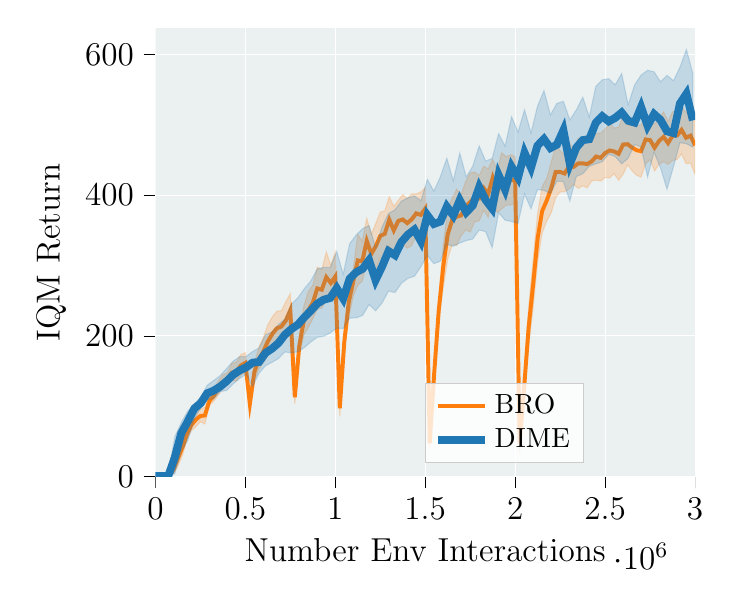
\begin{tikzpicture}

\definecolor{darkcyan1115178}{RGB}{1,115,178}
\definecolor{darkgray176}{RGB}{176,176,176}

\begin{axis}[
legend cell align={left},
legend cell align={left},
legend style={fill opacity=0.8, draw opacity=1, text opacity=1, draw=lightgray204, at={(0.5,0.03)},  anchor=south west},
tick align=outside,
tick pos=left,
x grid style={white},
xlabel={Number Env Interactions},
xmajorgrids,
%xmin=-149398.95, xmax=3000000.00,
xmin=0.0, xmax=3000000.00,
xtick style={color=black},
y grid style={white},
ylabel={IQM Return},
ymajorgrids,
%ymin=-37.9926843766667, ymax=923.09120151,
ymin=0.0, ymax=637.37269548,
ytick style={color=black},
axis background/.style={fill=plot_background},
label style={font=\large},
tick label style={font=\large},
x axis line style={draw=none},
y axis line style={draw=none},
]
% BRO

\path [draw=C1, fill=C1, opacity=0.2]
(axis cs:25000,1.06436189695316)
--(axis cs:25000,0.800044970854062)
--(axis cs:50000,0.902213431331389)
--(axis cs:75000,0.998039782938274)
--(axis cs:100000,3.73818093255901)
--(axis cs:125000,14.8008643633554)
--(axis cs:150000,29.8200848291147)
--(axis cs:175000,52.536500676349)
--(axis cs:200000,65.4528765036023)
--(axis cs:225000,70.6547353460924)
--(axis cs:250000,77.9210714654044)
--(axis cs:275000,74.6925274736162)
--(axis cs:300000,101.688198709863)
--(axis cs:325000,107.281306117989)
--(axis cs:350000,115.959467727732)
--(axis cs:375000,124.884927566366)
--(axis cs:400000,129.951946684364)
--(axis cs:425000,136.152626975576)
--(axis cs:450000,136.111337375472)
--(axis cs:475000,143.874927358078)
--(axis cs:500000,148.567262987423)
--(axis cs:525000,94.5117370449074)
--(axis cs:550000,137.525904720989)
--(axis cs:575000,152.664260638624)
--(axis cs:600000,161.929930494808)
--(axis cs:625000,171.58650975503)
--(axis cs:650000,181.142500891986)
--(axis cs:675000,186.720413352857)
--(axis cs:700000,191.754617425019)
--(axis cs:725000,196.874121030149)
--(axis cs:750000,212.645896156586)
--(axis cs:775000,103.542898066904)
--(axis cs:800000,171.614039449506)
--(axis cs:825000,201.242993560958)
--(axis cs:850000,211.747982944836)
--(axis cs:875000,224.177397591092)
--(axis cs:900000,237.999427608921)
--(axis cs:925000,239.436421657841)
--(axis cs:950000,250.973926888014)
--(axis cs:975000,250.707118365674)
--(axis cs:1000000,255.7721777332)
--(axis cs:1025000,85.7462506497815)
--(axis cs:1050000,177.039576732904)
--(axis cs:1075000,226.850952562221)
--(axis cs:1100000,256.461162193783)
--(axis cs:1125000,272.077354487363)
--(axis cs:1150000,277.88091019911)
--(axis cs:1175000,302.440032278388)
--(axis cs:1200000,286.286261722487)
--(axis cs:1225000,295.097707667798)
--(axis cs:1250000,310.062918562881)
--(axis cs:1275000,310.671213558559)
--(axis cs:1300000,328.891560548388)
--(axis cs:1325000,315.261131031065)
--(axis cs:1350000,333.264653443051)
--(axis cs:1375000,330.201890430345)
--(axis cs:1400000,324.50649705123)
--(axis cs:1425000,328.421995352062)
--(axis cs:1450000,343.634546505786)
--(axis cs:1475000,339.296630224071)
--(axis cs:1500000,348.984178695933)
--(axis cs:1525000,39.355588180581)
--(axis cs:1550000,132.834147960603)
--(axis cs:1575000,220.885853788656)
--(axis cs:1600000,268.221180119728)
--(axis cs:1625000,309.413007126434)
--(axis cs:1650000,330.020327352981)
--(axis cs:1675000,328.810183948437)
--(axis cs:1700000,342.485717291448)
--(axis cs:1725000,350.558346157369)
--(axis cs:1750000,347.543642435759)
--(axis cs:1775000,362.036408929491)
--(axis cs:1800000,363.429130292646)
--(axis cs:1825000,378.249045471367)
--(axis cs:1850000,368.466818930279)
--(axis cs:1875000,395.92381129835)
--(axis cs:1900000,375.255770601223)
--(axis cs:1925000,380.466843316452)
--(axis cs:1950000,385.742622584488)
--(axis cs:1975000,385.833705784746)
--(axis cs:2000000,388.274637595042)
--(axis cs:2025000,33.5649937116025)
--(axis cs:2050000,109.201720408668)
--(axis cs:2075000,186.449238204214)
--(axis cs:2100000,240.623289727134)
--(axis cs:2125000,305.664385445925)
--(axis cs:2150000,346.718313109583)
--(axis cs:2175000,362.847691076416)
--(axis cs:2200000,374.670521199756)
--(axis cs:2225000,396.743614451708)
--(axis cs:2250000,404.508816918751)
--(axis cs:2275000,404.815724919529)
--(axis cs:2300000,408.67455149964)
--(axis cs:2325000,415.555724534537)
--(axis cs:2350000,409.515642698911)
--(axis cs:2375000,413.456404646793)
--(axis cs:2400000,410.346599855339)
--(axis cs:2425000,420.13357683042)
--(axis cs:2450000,421.419850504902)
--(axis cs:2475000,420.083915472082)
--(axis cs:2500000,425.007581951612)
--(axis cs:2525000,424.579049671924)
--(axis cs:2550000,430.75366994294)
--(axis cs:2575000,421.216107533729)
--(axis cs:2600000,429.76793736549)
--(axis cs:2625000,443.105374475612)
--(axis cs:2650000,434.722857001578)
--(axis cs:2675000,428.275377228427)
--(axis cs:2700000,425.81611641096)
--(axis cs:2725000,444.64365130971)
--(axis cs:2750000,450.413269764893)
--(axis cs:2775000,434.345878022504)
--(axis cs:2800000,443.91301212502)
--(axis cs:2825000,447.49939896642)
--(axis cs:2850000,443.697419471331)
--(axis cs:2875000,449.354555033438)
--(axis cs:2900000,450.8026245623)
--(axis cs:2925000,458.680244532348)
--(axis cs:2950000,444.916782676853)
--(axis cs:2975000,445.634457360389)
--(axis cs:3000000,429.880019721412)
--(axis cs:3000000,513.9873176354)
--(axis cs:3000000,513.9873176354)
--(axis cs:2975000,523.797044053664)
--(axis cs:2950000,517.810496299027)
--(axis cs:2925000,525.954271943104)
--(axis cs:2900000,518.551529862146)
--(axis cs:2875000,518.920986906444)
--(axis cs:2850000,505.088500000573)
--(axis cs:2825000,518.566273395142)
--(axis cs:2800000,509.237923377759)
--(axis cs:2775000,501.25737445807)
--(axis cs:2750000,505.642689921167)
--(axis cs:2725000,513.254245513279)
--(axis cs:2700000,499.87053006485)
--(axis cs:2675000,499.068414301387)
--(axis cs:2650000,499.244308228539)
--(axis cs:2625000,500.18961766769)
--(axis cs:2600000,512.531552452399)
--(axis cs:2575000,496.697448428239)
--(axis cs:2550000,495.403692454602)
--(axis cs:2525000,502.740522809381)
--(axis cs:2500000,493.846745259791)
--(axis cs:2475000,488.320572719053)
--(axis cs:2450000,487.649215256229)
--(axis cs:2425000,478.718572892562)
--(axis cs:2400000,477.202876793975)
--(axis cs:2375000,476.451092629711)
--(axis cs:2350000,481.167057793168)
--(axis cs:2325000,464.822365433921)
--(axis cs:2300000,475.130801215997)
--(axis cs:2275000,457.275923790936)
--(axis cs:2250000,463.437629737087)
--(axis cs:2225000,469.693586932296)
--(axis cs:2200000,446.464641236289)
--(axis cs:2175000,423.741760297603)
--(axis cs:2150000,412.259115726332)
--(axis cs:2125000,374.619709027751)
--(axis cs:2100000,308.103900280336)
--(axis cs:2075000,240.504027337852)
--(axis cs:2050000,147.589375617486)
--(axis cs:2025000,60.8440314157716)
--(axis cs:2000000,454.6140241901)
--(axis cs:1975000,457.782889455546)
--(axis cs:1950000,454.490153888389)
--(axis cs:1925000,460.646195395525)
--(axis cs:1900000,435.379018582715)
--(axis cs:1875000,451.043381396628)
--(axis cs:1850000,437.594051329755)
--(axis cs:1825000,441.161889244782)
--(axis cs:1800000,428.1258205615)
--(axis cs:1775000,433.047391857064)
--(axis cs:1750000,431.680207172047)
--(axis cs:1725000,419.626783286342)
--(axis cs:1700000,401.334051733191)
--(axis cs:1675000,408.532521204368)
--(axis cs:1650000,395.947013655237)
--(axis cs:1625000,381.209360225348)
--(axis cs:1600000,328.600370144145)
--(axis cs:1575000,252.603144263693)
--(axis cs:1550000,162.227344584328)
--(axis cs:1525000,55.3468262239898)
--(axis cs:1500000,410.792177821071)
--(axis cs:1475000,404.502694934256)
--(axis cs:1450000,401.813256783996)
--(axis cs:1425000,401.708044362734)
--(axis cs:1400000,395.125789323197)
--(axis cs:1375000,400.825515156559)
--(axis cs:1350000,392.647754460344)
--(axis cs:1325000,384.152222205941)
--(axis cs:1300000,397.852872002416)
--(axis cs:1275000,377.552362447173)
--(axis cs:1250000,376.011972574837)
--(axis cs:1225000,359.739845675417)
--(axis cs:1200000,344.509178975306)
--(axis cs:1175000,367.154285866658)
--(axis cs:1150000,334.799456193374)
--(axis cs:1125000,344.307719911651)
--(axis cs:1100000,296.227318401859)
--(axis cs:1075000,266.643166383648)
--(axis cs:1050000,204.584202057326)
--(axis cs:1025000,108.689802307726)
--(axis cs:1000000,318.852715650748)
--(axis cs:975000,300.456149902442)
--(axis cs:950000,319.33259299771)
--(axis cs:925000,294.26813015175)
--(axis cs:900000,297.854696283069)
--(axis cs:875000,272.025279001709)
--(axis cs:850000,263.353273415112)
--(axis cs:825000,242.24173443444)
--(axis cs:800000,200.105312087152)
--(axis cs:775000,122.615578156031)
--(axis cs:750000,259.997946552285)
--(axis cs:725000,248.381254652691)
--(axis cs:700000,235.75254015339)
--(axis cs:675000,235.151123818793)
--(axis cs:650000,227.018726493552)
--(axis cs:625000,215.921378426131)
--(axis cs:600000,197.741080859391)
--(axis cs:575000,183.93247982137)
--(axis cs:550000,160.853477460561)
--(axis cs:525000,112.900779876465)
--(axis cs:500000,176.061616899139)
--(axis cs:475000,173.423721376022)
--(axis cs:450000,162.489487033554)
--(axis cs:425000,161.259046819264)
--(axis cs:400000,147.344859501089)
--(axis cs:375000,144.659394938876)
--(axis cs:350000,136.178883223972)
--(axis cs:325000,123.99330842961)
--(axis cs:300000,113.533585440671)
--(axis cs:275000,98.6956458394326)
--(axis cs:250000,95.6263797325166)
--(axis cs:225000,90.8477919575314)
--(axis cs:200000,80.6211055761968)
--(axis cs:175000,68.9779022961458)
--(axis cs:150000,52.6168055078161)
--(axis cs:125000,37.2068416693329)
--(axis cs:100000,17.4181970842278)
--(axis cs:75000,1.58356256613591)
--(axis cs:50000,1.25625000054544)
--(axis cs:25000,1.06436189695316)
--cycle;

\addplot [line width=\linewidthother, C1, mark=*, mark size=0, mark options={solid}]
table {%
25000 0.930442202091521
50000 1.07651185871321
75000 1.25993092696276
100000 9.83030688967838
125000 25.6411418517771
150000 41.1075536267594
175000 60.3883914444651
200000 73.172436582942
225000 80.957633586035
250000 86.0890838978233
275000 86.8321797068196
300000 107.266605289419
325000 114.972760323541
350000 125.514097446969
375000 134.324845411907
400000 138.233436327078
425000 147.660369336518
450000 148.782457916996
475000 157.754543249098
500000 161.480475192749
525000 103.279940413761
550000 148.67370118324
575000 166.636231776283
600000 177.730272953984
625000 192.167083171252
650000 202.772177321453
675000 210.734125891453
700000 213.205316409278
725000 221.706877576317
750000 236.467345033334
775000 112.87857606821
800000 186.130552121398
825000 221.723558177307
850000 236.209271737391
875000 247.087024794249
900000 267.471165250301
925000 265.658479214331
950000 283.439134541734
975000 275.133379987545
1000000 284.437051242526
1025000 97.0758468913518
1050000 191.453500474107
1075000 247.925237545804
1100000 277.620995193895
1125000 307.245282942146
1150000 305.919661019263
1175000 335.107741080569
1200000 316.435912664741
1225000 327.456512993191
1250000 342.107967490487
1275000 345.094845414729
1300000 365.251258681473
1325000 349.916712906547
1350000 363.318109792082
1375000 365.501578733968
1400000 360.257954947648
1425000 365.685379120745
1450000 374.145117409919
1475000 372.055178318366
1500000 380.772709979235
1525000 47.1556118690389
1550000 147.391608013536
1575000 235.725959616489
1600000 298.100854291553
1625000 344.459721335641
1650000 364.712840460148
1675000 369.42338730188
1700000 371.318808438126
1725000 383.874329652056
1750000 390.530684839555
1775000 396.82664916639
1800000 395.408529222678
1825000 409.974986250516
1850000 401.761351799987
1875000 424.544214100914
1900000 403.427991613482
1925000 421.452086824094
1950000 420.168662455335
1975000 421.239853255038
2000000 421.557400426789
2025000 46.8497645215133
2050000 127.574579390775
2075000 212.337561217824
2100000 273.695465882477
2125000 339.060702704761
2150000 377.404140539549
2175000 392.147298960786
2200000 409.585928423078
2225000 432.930123927388
2250000 433.06954152684
2275000 430.817714378362
2300000 441.242333227845
2325000 440.26544618574
2350000 445.109444370395
2375000 445.310468474792
2400000 444.23401205299
2425000 447.974403762188
2450000 455.009836622286
2475000 453.065691276495
2500000 459.824261297809
2525000 463.614242587133
2550000 462.153633274131
2575000 458.885605928128
2600000 472.045677739907
2625000 472.465960920779
2650000 467.617349708702
2675000 463.919322456368
2700000 462.572175194156
2725000 479.223260869987
2750000 478.300271910278
2775000 467.550224472069
2800000 477.243281641589
2825000 482.77498600685
2850000 474.021199131709
2875000 484.511658494648
2900000 484.88515836079
2925000 492.783683602026
2950000 481.675038930042
2975000 484.59483344476
3000000 470.838626791646
};
\addlegendentry{BRO}
% DIME
\path [draw=C0, fill=C0, opacity=0.2]
(axis cs:1,0.915501966666667)
--(axis cs:1,0.633556866666667)
--(axis cs:36000,0.5493304)
--(axis cs:72000,0.843873266666667)
--(axis cs:108000,4.13696455)
--(axis cs:144000,36.1211871666667)
--(axis cs:180000,51.4064937333333)
--(axis cs:216000,81.368514)
--(axis cs:252000,97.5408251666667)
--(axis cs:288000,109.583571666667)
--(axis cs:324000,110.618288333333)
--(axis cs:360000,120.684184666667)
--(axis cs:396000,122.417020833333)
--(axis cs:432000,131.747461666667)
--(axis cs:468000,139.23245)
--(axis cs:504000,145.708203333333)
--(axis cs:540000,128.071794166667)
--(axis cs:576000,146.743565)
--(axis cs:612000,157.523090333333)
--(axis cs:648000,162.386513333333)
--(axis cs:684000,167.712168333333)
--(axis cs:720000,177.17324)
--(axis cs:756000,175.778066666667)
--(axis cs:792000,177.557476666667)
--(axis cs:828000,183.413371666667)
--(axis cs:864000,191.343878333333)
--(axis cs:900000,198.058078333333)
--(axis cs:936000,199.495351666667)
--(axis cs:972000,204.18452)
--(axis cs:1008000,211.017165)
--(axis cs:1044000,210.395921666667)
--(axis cs:1080000,225.37889)
--(axis cs:1116000,225.57669)
--(axis cs:1152000,229.055506666667)
--(axis cs:1188000,244.717408333333)
--(axis cs:1224000,235.69925925)
--(axis cs:1260000,246.761671666667)
--(axis cs:1296000,263.70817)
--(axis cs:1332000,261.655338333333)
--(axis cs:1368000,274.904988333333)
--(axis cs:1404000,281.871765)
--(axis cs:1440000,284.6845)
--(axis cs:1476000,298.373705)
--(axis cs:1512000,314.234433333333)
--(axis cs:1548000,302.586606666667)
--(axis cs:1584000,306.158113166667)
--(axis cs:1620000,329.89694)
--(axis cs:1656000,327.346265)
--(axis cs:1692000,331.977616666667)
--(axis cs:1728000,335.598585)
--(axis cs:1764000,337.5854)
--(axis cs:1800000,350.510931458333)
--(axis cs:1836000,348.138216666667)
--(axis cs:1872000,325.377726666667)
--(axis cs:1908000,375.064071666667)
--(axis cs:1944000,364.504996666667)
--(axis cs:1980000,362.576775)
--(axis cs:2016000,359.905746666667)
--(axis cs:2052000,401.565295)
--(axis cs:2088000,380.944233333333)
--(axis cs:2124000,408.07439)
--(axis cs:2160000,406.816443333333)
--(axis cs:2196000,402.540623333333)
--(axis cs:2232000,419.828846666667)
--(axis cs:2268000,419.407693333333)
--(axis cs:2304000,391.893025)
--(axis cs:2340000,426.646173333333)
--(axis cs:2376000,430.59703)
--(axis cs:2412000,440.944021375)
--(axis cs:2448000,444.535958333333)
--(axis cs:2484000,447.59097)
--(axis cs:2520000,458.220718125)
--(axis cs:2556000,454.987311666667)
--(axis cs:2592000,444.593778333333)
--(axis cs:2628000,452.355353333333)
--(axis cs:2664000,472.315071583333)
--(axis cs:2700000,468.552297125)
--(axis cs:2736000,425.893185)
--(axis cs:2772000,461.17882)
--(axis cs:2808000,438.974565)
--(axis cs:2844000,408.566183333333)
--(axis cs:2880000,440.493023333333)
--(axis cs:2916000,474.594651666667)
--(axis cs:2952000,473.13282)
--(axis cs:2988000,468.31128725)
--(axis cs:2988000,572.54452975)
--(axis cs:2988000,572.54452975)
--(axis cs:2952000,607.047773333333)
--(axis cs:2916000,581.955683333333)
--(axis cs:2880000,562.69891)
--(axis cs:2844000,570.399441666667)
--(axis cs:2808000,561.294171666667)
--(axis cs:2772000,575.424046666667)
--(axis cs:2736000,577.564579375)
--(axis cs:2700000,570.731558333333)
--(axis cs:2664000,556.645568333333)
--(axis cs:2628000,528.610636666667)
--(axis cs:2592000,572.906766666667)
--(axis cs:2556000,556.792031666667)
--(axis cs:2520000,565.548321666667)
--(axis cs:2484000,564.076643333333)
--(axis cs:2448000,554.428711666667)
--(axis cs:2412000,511.028458333333)
--(axis cs:2376000,539.327213333333)
--(axis cs:2340000,521.274179458333)
--(axis cs:2304000,507.011033333333)
--(axis cs:2268000,533.545403333333)
--(axis cs:2232000,530.436551666667)
--(axis cs:2196000,514.156165)
--(axis cs:2160000,548.6599)
--(axis cs:2124000,526.241701666667)
--(axis cs:2088000,488.449933333333)
--(axis cs:2052000,521.397975)
--(axis cs:2016000,489.724498333333)
--(axis cs:1980000,511.56874)
--(axis cs:1944000,469.79517)
--(axis cs:1908000,487.4035)
--(axis cs:1872000,452.261116666667)
--(axis cs:1836000,448.443288333333)
--(axis cs:1800000,470.013476541667)
--(axis cs:1764000,441.067136666667)
--(axis cs:1728000,425.983283333333)
--(axis cs:1692000,459.900376666667)
--(axis cs:1656000,420.555463333333)
--(axis cs:1620000,452.412428333333)
--(axis cs:1584000,426.080911666667)
--(axis cs:1548000,405.744391916667)
--(axis cs:1512000,422.468795)
--(axis cs:1476000,392.121763333333)
--(axis cs:1440000,398.927006666667)
--(axis cs:1404000,396.300881666667)
--(axis cs:1368000,391.708926666667)
--(axis cs:1332000,379.3367)
--(axis cs:1296000,374.028266666667)
--(axis cs:1260000,354.826833333333)
--(axis cs:1224000,325.77437)
--(axis cs:1188000,356.78896)
--(axis cs:1152000,352.524811666667)
--(axis cs:1116000,343.294016666667)
--(axis cs:1080000,331.116815)
--(axis cs:1044000,287.783165)
--(axis cs:1008000,319.938826666667)
--(axis cs:972000,297.00894)
--(axis cs:936000,297.43841)
--(axis cs:900000,295.160138333333)
--(axis cs:864000,278.186283333333)
--(axis cs:828000,267.117865)
--(axis cs:792000,254.04739775)
--(axis cs:756000,245.040613333333)
--(axis cs:720000,223.696456875)
--(axis cs:684000,216.1656)
--(axis cs:648000,205.401713333333)
--(axis cs:612000,201.404601666667)
--(axis cs:576000,182.55503)
--(axis cs:540000,177.786793333333)
--(axis cs:504000,170.561265208333)
--(axis cs:468000,170.450261666667)
--(axis cs:432000,164.02998)
--(axis cs:396000,153.633991666667)
--(axis cs:360000,143.37209)
--(axis cs:324000,136.525775833333)
--(axis cs:288000,129.716861683333)
--(axis cs:252000,113.1404125)
--(axis cs:216000,102.49002)
--(axis cs:180000,92.9197603333333)
--(axis cs:144000,76.8890066666667)
--(axis cs:108000,56.7536433333333)
--(axis cs:72000,4.25857906666667)
--(axis cs:36000,0.728938933333333)
--(axis cs:1,0.915501966666667)
--cycle;

\addplot [line width=\linewidthdime, C0, mark=*, mark size=0, mark options={solid}]
table {%
1 0.770562166666667
36000 0.658370533333333
72000 1.02744053333333
108000 27.4132359166667
144000 61.7389005
180000 78.3388245
216000 96.6475441666667
252000 104.292225666667
288000 118.336289333333
324000 122.156900833333
360000 127.865645666667
396000 135.589655833333
432000 144.61231
468000 150.876916666667
504000 155.106371666667
540000 161.848961666667
576000 162.873085
612000 175.66877
648000 181.774033333333
684000 189.795443333333
720000 201.694543333333
756000 209.679653333333
792000 215.950858333333
828000 226.452128333333
864000 235.790758333333
900000 245.745095
936000 251.419853333333
972000 253.923228333333
1008000 267.745066666667
1044000 253.029908333333
1080000 281.1757
1116000 290.478148333333
1152000 295.386573333333
1188000 307.510898333333
1224000 279.324226666667
1260000 298.499671666667
1296000 320.530285
1332000 314.688511666667
1368000 333.564955
1404000 344.035705
1440000 351.026203333333
1476000 334.48205
1512000 371.517083333333
1548000 359.107073333333
1584000 362.49581
1620000 383.735268333333
1656000 371.120853333333
1692000 392.875408333333
1728000 375.706403333333
1764000 385.148411666667
1800000 411.377563333333
1836000 393.022041666667
1872000 381.083618333333
1908000 428.514751666667
1944000 407.976545
1980000 440.522148333333
2016000 425.096363333333
2052000 460.246375
2088000 439.221346666667
2124000 470.482476666667
2160000 479.806223333333
2196000 467.028006666667
2232000 471.833656666667
2268000 492.305195
2304000 444.283438333333
2340000 467.734686666667
2376000 478.305563333333
2412000 479.659883333333
2448000 502.891963333333
2484000 512.254108333333
2520000 504.927955
2556000 509.89631
2592000 517.465808333333
2628000 505.843831666667
2664000 503.219516666667
2700000 525.334166666667
2736000 498.718568333333
2772000 515.273173333333
2808000 507.004858333333
2844000 490.845221666667
2880000 488.33129
2916000 530.288801666667
2952000 544.121438333333
2988000 506.351106666667
};
\addlegendentry{DIME}
\end{axis}

\end{tikzpicture}
}
       \subcaption[]{DIME and BRO on Humanoid Run}
       \label{fig::appendix_dime_bro_humanoid_run_long}
    \end{minipage}\hfill
    \caption{\textbf{Preliminary results for the GB sampler on the dog run (a) and humanoid run (b) environments from DMC. 
    Comparison to BRO on the humanoid run for 3 million steps. 
    }
    }
    \label{fig::appendix::prel::dbs}
\end{figure*}



%%%%%%%%%%%%%%%%%%%%%%%%%%%%%%%%%%%%%%%%%%%%%%%%%%%%%%%%%%%%%%%%%%%%%%%
\begin{figure*}[t!]
        \centering
        \begin{minipage}[t!]{\textwidth}
            \centering
            \begin{minipage}[t!]{0.32\textwidth}
            \includegraphics[width=\textwidth]{figures/illustrations/small_entropy.pdf}
            \subcaption[]{$\ \alpha < 1$}
            \end{minipage}
            \begin{minipage}[t!]{0.32\textwidth}
            \includegraphics[width=\textwidth]{figures/illustrations/normal_entropy.pdf}
            \subcaption[]{$\ \alpha = 1$}
            \end{minipage}
            \begin{minipage}[t!]{0.32\textwidth}
            \includegraphics[width=\textwidth]{figures/illustrations/big_entropy.pdf}
            \subcaption[]{$\ \alpha > 1$}
            \end{minipage}
        \end{minipage}
        \caption[ ]
        {\textbf{The effect of the reward scaling parameter $\alpha$}. The figures in (a)-(b) show diffusion processes for different $\alpha$ values starting at a prior distribution $\mathcal{N}(0,I)$ and going backward in time to approximate the target distribution $\exp{\left(Q^\pi/\alpha\right)}/Z^\pi$. Small values for $\alpha$ (a) lead to concentrated target distributions with less noise in the diffusion trajectories especially at the last time steps. The higher $\alpha$ becomes (b) and (c), the more the target distribution is smoothed and the distribution of the samples at the last time steps becomes more noisy. Therefore, the parameter $\alpha$ directly controls the exploration by enforcing noisier samples the higher $\alpha$ becomes.}
        \label{fig:entropies}
    \end{figure*}
%%%%%%%%%%%%%%%%%%%%%%%%%%%%%%%%%%%%%%%%%%%%%%%%%%%%%%%%%%%%%%%%%%%%%%%



%%%%%%%%%%%%%%%%%%%%%%%%%%%%%%%%%%%%%%%%%%%%%%%%%%%%%%%%%%%%%%%%%%%%%%%%%%%%%%%
%%%%%%%%%%%%%%%%%%%%%%%%%%%%%%%%%%%%%%%%%%%%%%%%%%%%%%%%%%%%%%%%%%%%%%%%%%%%%%%


\end{document}


% This document was modified from the file originally made available by
% Pat Langley and Andrea Danyluk for ICML-2K. This version was created
% by Iain Murray in 2018, and modified by Alexandre Bouchard in
% 2019 and 2021 and by Csaba Szepesvari, Gang Niu and Sivan Sabato in 2022.
% Modified again in 2023 and 2024 by Sivan Sabato and Jonathan Scarlett.
% Previous contributors include Dan Roy, Lise Getoor and Tobias
% Scheffer, which was slightly modified from the 2010 version by
% Thorsten Joachims & Johannes Fuernkranz, slightly modified from the
% 2009 version by Kiri Wagstaff and Sam Roweis's 2008 version, which is
% slightly modified from Prasad Tadepalli's 2007 version which is a
% lightly changed version of the previous year's version by Andrew
% Moore, which was in turn edited from those of Kristian Kersting and
% Codrina Lauth. Alex Smola contributed to the algorithmic style files.
